% deepstudy-pdf — Roadmap de Domínio: TypeScript + JavaScript (v2)
\documentclass[12pt,a4paper,oneside]{book}
\usepackage[utf8]{inputenc}
\usepackage[T1]{fontenc}
\usepackage{amsmath,amssymb}
\usepackage{listings}
\usepackage{xcolor}
\usepackage{hyperref}
\usepackage{tikz}
\usetikzlibrary{arrows.meta}
\usetikzlibrary{shapes.geometric}
\usetikzlibrary{positioning}
\usepackage{minted}
\usepackage{tcolorbox}
\usepackage{geometry}
\usepackage{fancyhdr}
\usepackage{imakeidx}
\usepackage{booktabs}
\usepackage{tabularx}

\makeindex[intoc]

\geometry{margin=2.5cm}
\setlength{\parskip}{0.8em}
\setlength{\parindent}{0pt}

\setminted{linenos, frame=single, breaklines, fontsize=\small, numbersep=6pt, tabsize=2}

\pagestyle{fancy}
\fancyhf{}
\fancyhead[LE,RO]{\thepage}
\fancyhead[RE]{\nouppercase{\leftmark}}
\fancyhead[LO]{\nouppercase{\rightmark}}

\hypersetup{
    colorlinks=true,
    linkcolor=blue!60!black,
    urlcolor=blue!60!black,
    citecolor=blue!60!black,
}

% ---- marcadores de prioridade e caixas ----
\newcommand{\alta}{\colorbox{red!15}{\sffamily\scriptsize\bfseries PRIORIDADE ALTA}}
\newcommand{\media}{\colorbox{orange!20}{\sffamily\scriptsize\bfseries PRIORIDADE MÉDIA}}
\newcommand{\baixa}{\colorbox{gray!20}{\sffamily\scriptsize\bfseries PRIORIDADE BAIXA}}
\newcommand{\Ta}{\textcolor{red!70!black}{\sffamily\bfseries Alta}}
\newcommand{\Tm}{\textcolor{orange!80!black}{\sffamily\bfseries Média}}
\newcommand{\Tb}{\textcolor{gray}{\sffamily\bfseries Baixa}}
\newcommand{\code}[1]{\texttt{#1}}
\newcommand{\cb}{$\square$}
\newtcolorbox{nota}[1][Nota]{colback=blue!3,colframe=blue!50!black,title={#1},fonttitle=\bfseries,boxrule=0.6pt,arc=2pt}
\newtcolorbox{cuidado}[1][Cuidado]{colback=orange!5,colframe=orange!70!black,title={#1},fonttitle=\bfseries,boxrule=0.6pt,arc=2pt}
\newtcolorbox{projeto}[1]{colback=gray!4,colframe=black!60,title={#1},fonttitle=\bfseries,boxrule=0.6pt,arc=2pt}
\newtcolorbox{dominio}{colback=green!4,colframe=green!45!black,boxrule=0.6pt,arc=2pt,left=4pt,right=4pt,top=2pt,bottom=2pt}
\newcommand{\dom}[1]{\begin{dominio}\textbf{Domínio:} #1\end{dominio}}

\tikzset{
  caixa/.style={draw, rounded corners=2pt, fill=gray!8, align=center, text width=#1, inner sep=4pt, font=\small},
  caixa/.default=2.4cm,
  seta/.style={-Stealth, thick},
}

\title{Roadmap de Domínio --- TypeScript + JavaScript\\[0.4em]\Large Do runtime ao compile time: um guia prático para desenvolvedores backend}
\author{DeepStudy PDF Generator}
\date{\today}

\begin{document}

\maketitle
\tableofcontents

% =====================================================================
\chapter*{Como usar este documento}
\addcontentsline{toc}{chapter}{Como usar este documento}
\markboth{Como usar este documento}{Como usar este documento}

Este documento \textbf{não é um livro didático}. É um \textbf{checklist de estudos e um mapa de prioridades} para desenvolvedores que já escrevem código e querem consolidar TypeScript como linguagem principal, entendendo o JavaScript que roda por baixo.

\section*{Ficha do roadmap}

\begin{tabularx}{\textwidth}{@{}lX@{}}
\toprule
\textbf{Foco} & 70\% TypeScript, 30\% JavaScript \\
\textbf{Nível} & pleno consolidando stack backend \\
\textbf{Stack} & Node.js, TypeScript, backend \\
\textbf{Formato} & checklist de estudos e mapa de prioridades \\
\textbf{Duração sugerida} & 3 a 6 meses com dedicação consistente \\
\textbf{Licença} & CC BY-NC-SA 4.0 \\
\bottomrule
\end{tabularx}

\section*{Como navegar}

\begin{itemize}
  \item Use o sumário para ir direto a uma seção.
  \item Marque os checkboxes do Capítulo~\ref{cap:checklist} conforme dominar cada tópico.
  \item A ordem sugerida está no Capítulo~\ref{cap:ordem}, mas pode ser adaptada ao seu contexto.
  \item Cada tópico tem uma \textbf{marca de prioridade} e termina com uma caixa \textbf{Domínio}: um critério verificável para saber se você realmente aprendeu.
\end{itemize}

\section*{Legenda de prioridade}

\begin{tabularx}{\textwidth}{@{}lX@{}}
\toprule
\alta & Estude \textbf{primeiro}. Essencial para o dia a dia; sem isso o TypeScript vira um conjunto de regras decoradas. \\
\media & Estude \textbf{depois de consolidar o essencial} ou quando aparecer no projeto. \\
\baixa & Útil, mas não bloqueia nada. Adie sem culpa e aprofunde sob demanda. \\
\bottomrule
\end{tabularx}

\section*{Pré-requisitos assumidos}

\begin{itemize}
  \item Git básico (commit, branch, merge);
  \item terminal/shell (navegação, variáveis de ambiente);
  \item Node.js instalado (versão LTS atual);
  \item editor configurado (VS Code recomendado, com o TypeScript do workspace);
  \item noções de HTTP e APIs REST;
  \item familiaridade com \code{npm} ou \code{pnpm}.
\end{itemize}

\section*{As seis perguntas que este documento responde}

\begin{tabularx}{\textwidth}{@{}rXl@{}}
\toprule
\# & Pergunta & Onde \\
\midrule
1 & O que preciso saber de JavaScript para dominar TypeScript? & Cap.~\ref{cap:js} \\
2 & O que devo estudar primeiro? & Caps.~\ref{cap:js} e~\ref{cap:ordem} \\
3 & O que posso deixar para depois? & Seções~\ref{sec:jsbaixa} e~\ref{cap:tsavancado} \\
4 & Quais assuntos são especificamente de TypeScript? & Caps.~\ref{cap:tsnucleo},~\ref{cap:tsavancado} e~\ref{cap:ferramentas} \\
5 & Quais assuntos de Node.js complementam esse conhecimento? & Cap.~\ref{cap:node} \\
6 & Como saber se realmente dominei cada tópico? & Cap.~\ref{cap:checklist} \\
\bottomrule
\end{tabularx}

% =====================================================================
\chapter{Introdução: compile time e runtime}

A distinção fundamental que organiza todo este roadmap:

\begin{quote}
\textbf{TypeScript existe principalmente em compile time, enquanto JavaScript é o que efetivamente executa em runtime.}
\end{quote}

O TypeScript é um sistema de tipos estático sobre o JavaScript. O compilador lê o código, verifica se os tipos são coerentes e depois \textbf{apaga os tipos}\index{type erasure} (\emph{type erasure}). O que chega ao Node.js é JavaScript puro.

\begin{minted}{typescript}
function pegarNome(usuario: { nome: string }) {
  return usuario.nome;
}
\end{minted}

Depois da compilação:

\begin{minted}{javascript}
function pegarNome(usuario) {
  return usuario.nome;
}
\end{minted}

\begin{figure}[h]
\centering
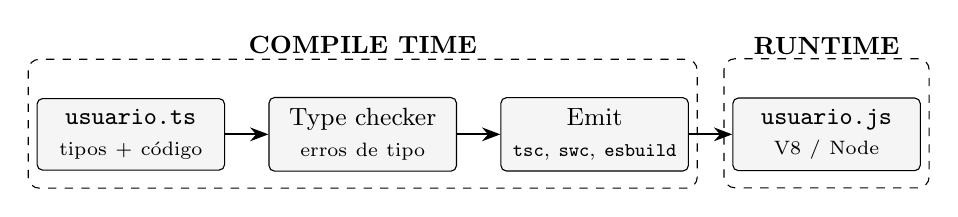
\begin{tikzpicture}[node distance=0.55cm]
  \node[caixa=2.1cm] (ts) {\texttt{usuario.ts}\\\scriptsize tipos + código};
  \node[caixa=2.1cm, right=of ts] (chk) {Type checker\\\scriptsize erros de tipo};
  \node[caixa=2.1cm, right=of chk] (emit) {Emit\\\scriptsize\texttt{tsc}, \texttt{swc}, \texttt{esbuild}};
  \node[caixa=2.1cm, right=of emit] (js) {\texttt{usuario.js}\\\scriptsize V8 / Node};
  \draw[seta] (ts) -- (chk);
  \draw[seta] (chk) -- (emit);
  \draw[seta] (emit) -- (js);
  \draw[dashed, rounded corners] ([xshift=-3pt,yshift=14pt]ts.north west) rectangle ([xshift=3pt,yshift=-6pt]emit.south east);
  \node[above=12pt of chk, font=\small\bfseries] {COMPILE TIME};
  \draw[dashed, rounded corners] ([xshift=-3pt,yshift=14pt]js.north west) rectangle ([xshift=3pt,yshift=-6pt]js.south east);
  \node[above=12pt of js, font=\small\bfseries] {RUNTIME};
\end{tikzpicture}
\caption{Os tipos existem até o emit. Tudo o que acontece depois, inclusive os bugs de runtime, é JavaScript sem tipos e sem garantias.}
\end{figure}

A consequência é direta: o TypeScript fornece \textbf{garantias estáticas}, mas \textbf{não altera o comportamento do JavaScript em runtime}. Ele não valida o body de uma requisição, não converte tipos e não impede que um \code{JSON.parse} devolva algo diferente do declarado. Sem entender o comportamento real do JS (closures, \code{this}, prototype, Event Loop, coerção), você escreve TypeScript que \emph{parece} correto e quebra em produção:

\begin{minted}{typescript}
type Usuario = { nome: string };

const body = '{"nome": 42}';                 // veio da rede
const usuario = JSON.parse(body) as Usuario; // "confie em mim, compilador"

usuario.nome.toUpperCase();
// compila sem erros -- e em runtime:
// TypeError: usuario.nome.toUpperCase is not a function
\end{minted}

\begin{nota}[Modelo mental]
Os tipos são uma \textbf{descrição} do que você espera que o JavaScript faça. Quando descrição e realidade divergem, o runtime vence. Por isso dominar TypeScript exige entender o JavaScript por baixo dele --- e validar em runtime tudo o que vem de fora (Seção~\ref{sec:validacao}).
\end{nota}

\begin{nota}[Recursos que geram código]
Alguns recursos do TS \emph{emitem} JavaScript: \code{enum}, \code{namespace} com valores, parameter properties (\code{constructor(private x: T)}) e decorators. A execução nativa de \code{.ts} pelo Node (\emph{type stripping}) e a flag \code{erasableSyntaxOnly} rejeitam os que não podem ser simplesmente apagados.
\end{nota}

% =====================================================================
\chapter{Estratégia de estudo}

\begin{tabularx}{\textwidth}{@{}lX@{}}
\toprule
\textbf{70\% TypeScript} & Foco principal, onde o tempo é investido: modelagem com tipos, narrowing, generics, tipos derivados, ferramentas e configuração. \\
\textbf{30\% JavaScript} & Fundamento, estudado conforme sustenta o TS: escopo, closures, \code{this}, referências, erros, async, Event Loop, prototype. \\
\textbf{0\%} & Detalhes históricos e quirks obscuros. \\
\bottomrule
\end{tabularx}

Você \textbf{não precisa} dominar todos os detalhes históricos ou obscuros do JavaScript para dominar TypeScript. Tabelas de coerção do \code{==}, \code{with} ou as idiossincrasias de \code{Date} não mudam como você modela tipos. O que muda é entender \textbf{de onde vêm os valores e como eles se comportam}.

\begin{quote}
\textbf{Estratégia:} aprender TypeScript e estudar JavaScript conforme ele explica o comportamento do código TypeScript.
\end{quote}

Na prática: se você está estudando generics e surge uma dúvida sobre closures, pare e estude closures. A motivação vem do uso, não de uma trilha linear exaustiva.

\begin{figure}[h]
\centering
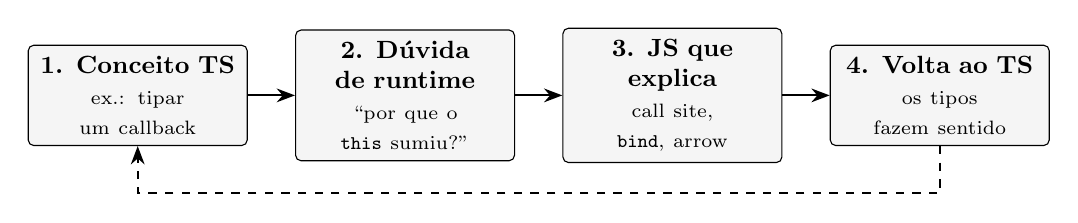
\begin{tikzpicture}[node distance=0.6cm]
  \node[caixa=2.5cm] (a) {\textbf{1. Conceito TS}\\\scriptsize ex.: tipar um callback};
  \node[caixa=2.5cm, right=of a] (b) {\textbf{2. Dúvida de runtime}\\\scriptsize ``por que o \texttt{this} sumiu?''};
  \node[caixa=2.5cm, right=of b] (c) {\textbf{3. JS que explica}\\\scriptsize call site, \texttt{bind}, arrow};
  \node[caixa=2.5cm, right=of c] (d) {\textbf{4. Volta ao TS}\\\scriptsize os tipos fazem sentido};
  \draw[seta] (a) -- (b); \draw[seta] (b) -- (c); \draw[seta] (c) -- (d);
  \draw[seta, dashed] (d.south) -- ++(0,-0.6) -| (a.south);
\end{tikzpicture}
\caption{O ciclo de estudo: o TypeScript puxa o JavaScript que for necessário.}
\end{figure}

\section{Estimativa de tempo}

\begin{center}
\begin{tabular}{@{}ll@{}}
\toprule
\textbf{Bloco} & \textbf{Tempo estimado} \\
\midrule
JavaScript essencial & 4--6 semanas \\
TypeScript: fundamentos até generics & 6--8 semanas \\
TypeScript avançado & 4--6 semanas \\
Ferramentas e ecossistema & 2--3 semanas \\
Node.js internals & 4--6 semanas \\
Prática contínua com projetos & em paralelo, sempre \\
\midrule
\textbf{Total sugerido} & \textbf{3 a 6 meses} com dedicação consistente \\
\bottomrule
\end{tabular}
\end{center}

Os blocos se sobrepõem: o total é menor que a soma porque JavaScript e TypeScript são estudados em paralelo.

\section{Mapa: conceito de TS e o JavaScript que o explica}

{\small
\begin{tabularx}{\textwidth}{@{}XXX@{}}
\toprule
\textbf{No TypeScript você estuda\ldots} & \textbf{\ldots o JS que explica é} & \textbf{Por quê} \\
\midrule
Tipos de funções, generics em callbacks & Funções de primeira classe, closures & O tipo descreve uma função que captura estado \\
\code{typeof}, \code{instanceof}, \code{in} & Operadores de runtime, prototype chain & Narrowing é o TS lendo checagens reais \\
Classes, \code{private}, \code{\#campo} & Prototype, class fields & \code{private} some no emit; \code{\#} existe em runtime \\
\code{Promise<T>}, \code{Awaited} & Promises, Event Loop & O tipo descreve o valor futuro, não quando ele chega \\
\code{readonly}, \code{Readonly<T>} & Referências, mutabilidade & \code{readonly} é só compile time e é raso \\
\code{keyof}, indexed access & Objetos, propriedades dinâmicas & \code{obj[chave]} é JS; o TS tipa a chave \\
Parâmetro \code{this} & Regras de binding de \code{this} & O TS modela uma regra resolvida no call site \\
\code{catch (err: unknown)} & Tratamento de erros & Em JS qualquer valor pode ser lançado \\
\code{import type}, \code{module} & ESM e CommonJS & O \code{tsconfig} precisa refletir o runtime \\
\bottomrule
\end{tabularx}
}

% =====================================================================
\chapter{JavaScript essencial para dominar TypeScript}
\label{cap:js}

As seções~\ref{sec:scope} a~\ref{sec:prototype} são \alta: elas explicam praticamente todo bug de runtime que o TypeScript não pega. Estude na ordem. Os tópicos de prioridade média e baixa estão no fim do capítulo.

\section{Scope e Lexical Scope}
\label{sec:scope}
\index{lexical scope}
\alta

\begin{itemize}
  \item escopo global, de função e de bloco;
  \item \code{let}, \code{const} e \code{var} --- diferenças reais;
  \item lexical environment e bindings;
  \item Temporal Dead Zone (TDZ)\index{TDZ} e hoisting\index{hoisting}.
\end{itemize}

\textbf{Lexical scope} significa que o escopo é decidido por \emph{onde a função foi escrita}, não por onde ela é chamada. Cada bloco ou função cria um \emph{lexical environment}\index{lexical environment}: uma tabela de \textbf{bindings} (nome $\rightarrow$ valor) mais uma referência para o ambiente externo.

\begin{minted}{javascript}
console.log(a); // undefined -- var é hoisted e inicializado com undefined
console.log(b); // ReferenceError -- b está na TDZ até a declaração
var a = 1;          // escopo de função (ou global)
let b = 2;          // escopo de bloco
const c = { n: 3 }; // o BINDING é constante -- o objeto continua mutável

if (true) {
  var x = 'vaza';   // pertence à função/módulo, não ao bloco
  let y = 'fica';   // pertence ao bloco
}
console.log(x); // 'vaza'
console.log(y); // ReferenceError: y is not defined
c.n = 4;        // ok
c = {};         // TypeError: Assignment to constant variable.
\end{minted}

\begin{figure}[h]
\centering
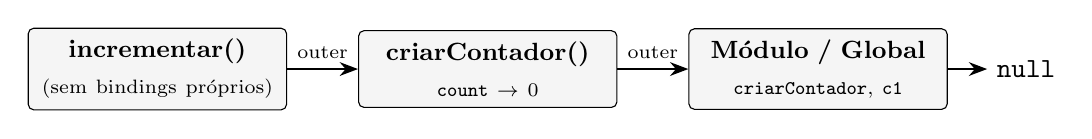
\begin{tikzpicture}[node distance=0.9cm]
  \node[caixa=3cm] (inc) {\textbf{incrementar()}\\[2pt]\scriptsize (sem bindings próprios)};
  \node[caixa=3cm, right=of inc] (cc) {\textbf{criarContador()}\\[2pt]\scriptsize\texttt{count} $\rightarrow$ 0};
  \node[caixa=3cm, right=of cc] (glob) {\textbf{Módulo / Global}\\[2pt]\scriptsize\texttt{criarContador}, \texttt{c1}};
  \node[right=0.5cm of glob] (null) {\texttt{null}};
  \draw[seta] (inc) -- node[above, font=\scriptsize]{outer} (cc);
  \draw[seta] (cc) -- node[above, font=\scriptsize]{outer} (glob);
  \draw[seta] (glob) -- (null);
\end{tikzpicture}
\caption{Cadeia de lexical environments. Para resolver \texttt{count} dentro de \texttt{incrementar()}, o JS procura no ambiente atual e sobe pela referência \emph{outer} até encontrar; se chegar a \texttt{null}, lança \texttt{ReferenceError}.}
\end{figure}

\dom{você explica a diferença entre TDZ e o hoisting de \code{var} e prevê o resultado de qualquer trecho com blocos aninhados sem executar.}

\section{Closures}
\label{sec:closures}
\index{closure}
\alta

\begin{itemize}
  \item conceito e por que existem;
  \item funções retornadas e estado privado;
  \item closures em loops e a diferença entre \code{let} e \code{var};
  \item factory functions\index{factory function}.
\end{itemize}

Uma \textbf{closure} é uma função mais o lexical environment em que ela foi criada. Se a função sobrevive à execução de quem a criou, o ambiente sobrevive junto. É o mecanismo por trás de estado privado e de factory functions.

\begin{minted}{javascript}
function criarContador() {
  let count = 0;                 // ninguém de fora acessa diretamente
  return {
    incrementar: () => ++count,
    atual: () => count,
  };
}

const c1 = criarContador();
c1.incrementar();
c1.incrementar();
c1.atual();   // 2

const c2 = criarContador();
c2.atual();   // 0 -- cada chamada cria um NOVO ambiente
\end{minted}

\begin{figure}[h]
\centering
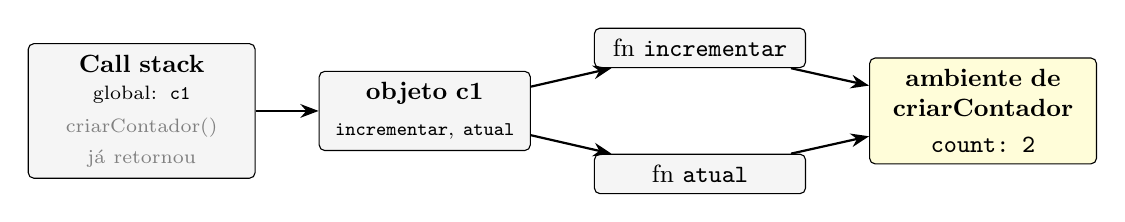
\begin{tikzpicture}[node distance=0.8cm]
  \node[caixa=2.6cm] (stack) {\textbf{Call stack}\\[2pt]\scriptsize global: \texttt{c1}\\[1pt]\scriptsize\textcolor{gray}{criarContador() já retornou}};
  \node[caixa=2.4cm, right=of stack] (obj) {\textbf{objeto c1}\\[2pt]\scriptsize\texttt{incrementar}, \texttt{atual}};
  \node[caixa=2.4cm, right=of obj, yshift=0.8cm] (f1) {fn \texttt{incrementar}};
  \node[caixa=2.4cm, right=of obj, yshift=-0.8cm] (f2) {fn \texttt{atual}};
  \node[caixa=2.6cm, right=of f1, yshift=-0.8cm, fill=yellow!15] (env) {\textbf{ambiente de criarContador}\\[2pt]\texttt{count: 2}};
  \draw[seta] (stack) -- (obj);
  \draw[seta] (obj) -- (f1); \draw[seta] (obj) -- (f2);
  \draw[seta] (f1) -- (env);
  \draw[seta] (f2) -- (env);
\end{tikzpicture}
\caption{O frame de \texttt{criarContador()} saiu da pilha, mas o ambiente com \texttt{count} continua vivo no heap enquanto alguma função apontar para ele (as setas à direita são o link interno \texttt{[[Environment]]} de cada função).}
\end{figure}

A pergunta clássica sobre closures em loops:

\begin{minted}{javascript}
for (var i = 0; i < 3; i++) setTimeout(() => console.log(i)); // 3 3 3
for (let j = 0; j < 3; j++) setTimeout(() => console.log(j)); // 0 1 2
// var: UM binding compartilhado pelo loop inteiro.
// let: um binding NOVO por iteração -- cada callback captura o seu.
\end{minted}

\dom{você escreve uma factory com estado privado (por exemplo, um rate limiter em memória) sem hesitar, explica o \code{3 3 3} e sabe que closures retêm memória enquanto forem referenciadas.}

\section{\texttt{this}}
\label{sec:this}
\index{this}
\alta

O valor de \code{this} é decidido no \textbf{call site}, isto é, na forma como a função é chamada, e não onde ela foi definida. Arrow functions são a exceção: não têm \code{this} próprio e herdam o do escopo léxico.

\begin{minted}{javascript}
const conta = {
  saldo: 100,
  ver() { return this.saldo; },
  verArrow: () => this?.saldo,   // this léxico do módulo -> undefined
};

conta.ver();                     // 100 -- call site: conta.ver()
const solta = conta.ver;
solta();                         // TypeError: this é undefined (strict mode)
solta.call({ saldo: 5 });        // 5
solta.apply({ saldo: 7 }, []);   // 7 (argumentos como array)
const presa = conta.ver.bind(conta);
presa();                         // 100
conta.verArrow();                // undefined -- arrow ignora o call site
\end{minted}

\begin{center}
\begin{tabular}{@{}lll@{}}
\toprule
\textbf{Forma de chamar} & \textbf{Função normal} & \textbf{Arrow function} \\
\midrule
\code{obj.f()} & \code{obj} & \code{this} de onde foi definida \\
\code{f()} & \code{undefined} (strict) / global (sloppy) & idem \\
\code{f.call(x)} / \code{f.apply(x, args)} & \code{x} & ignora \code{x} \\
\code{f.bind(x)()} & \code{x} (fixo) & ignora \code{x} \\
\code{new F()} & novo objeto & erro: não é construtor \\
\bottomrule
\end{tabular}
\end{center}

\begin{cuidado}[Bug real de backend]
\code{router.get('/pedidos', controller.listar)} passa o método \emph{solto}: dentro dele, \code{this.service} é \code{undefined}. Soluções: \code{controller.listar.bind(controller)}, \code{(req, res) => controller.listar(req, res)} ou declarar o método como arrow property.
\end{cuidado}

\dom{dado qualquer call site, você diz o valor de \code{this}; sabe quando \code{bind} é necessário e quando \emph{não} usar arrow functions (métodos de protótipo, construtores).}

\section{Objetos e referências}
\label{sec:objetos}
\alta

Primitivos são copiados por valor; objetos, arrays e funções são manipulados por \textbf{referência}. Spread faz \textbf{shallow copy}\index{shallow copy}: o primeiro nível é novo, os objetos aninhados continuam compartilhados.

\begin{minted}{javascript}
const a = { nome: 'Ana', endereco: { cidade: 'POA' } };
const b = a;                  // mesma referência: b === a
const c = { ...a };           // shallow copy (equivale a Object.assign({}, a))
c.nome = 'Bia';               // não afeta a
c.endereco.cidade = 'SP';     // AFETA a.endereco -- objeto aninhado compartilhado
const d = structuredClone(a); // deep copy (Node 17+)

Object.freeze(a);  // não permite adicionar, remover nem alterar (raso!)
Object.seal(a);    // permite alterar, mas não adicionar nem remover
a.endereco.cidade = 'RJ';     // funciona mesmo com freeze: freeze é raso

const { nome, endereco: { cidade }, ...resto } = a;  // destructuring + rest
function salvar({ id, ...dados }) { /* ... */ }       // destructuring em parâmetro
\end{minted}

\begin{nota}[Conexão com TypeScript]
\code{readonly} e \code{Readonly<T>} são rasos e só existem em compile time. Outra referência sem \code{readonly} pode mutar o mesmo objeto. Para imutabilidade em runtime, use \code{Object.freeze} (também raso).
\end{nota}

\dom{você identifica mutação acidental por referência compartilhada (por exemplo, um objeto default reaproveitado entre requisições) e escolhe conscientemente entre spread, \code{Object.freeze} e \code{structuredClone}.}

\section{Funções}
\label{sec:funcoes}
\index{função de ordem superior}
\alta

Funções de primeira classe, callbacks, funções de ordem superior (HOF), parâmetros rest, default parameters e tagged templates.

\begin{minted}{javascript}
const aplicar = (fn, ...args) => fn(...args);  // rest na definição, spread na chamada

function saudar(nome = 'mundo') {             // default dispara só para undefined
  return `olá, ${nome}`;
}

const comLog = (fn) => (...args) => {          // HOF: recebe e devolve função
  console.log('chamando', fn.name, args);
  return fn(...args);
};

// tagged template: a função recebe as partes fixas e os valores separados
function sql(partes, ...valores) {
  return { texto: partes.join('?'), valores };  // base de libs de SQL seguras
}
sql`SELECT * FROM pedidos WHERE id = ${id} AND status = ${status}`;
// { texto: 'SELECT * FROM pedidos WHERE id = ? AND status = ?', valores: [id, status] }
\end{minted}

\dom{você escreve um wrapper de função (log, retry, cache) como HOF, sabe que default parameters não disparam para \code{null} e explica por que tagged templates evitam SQL injection.}

\section{Arrays}
\label{sec:arrays}
\alta

Domine sem consultar \code{map}, \code{filter}, \code{reduce}, \code{find}, \code{findIndex}, \code{some}, \code{every}, \code{sort}, \code{flat}, \code{flatMap} e \code{at}, e saiba quais deles \textbf{mutam} o array original.

\begin{minted}{javascript}
const pedidos = [
  { id: 1, cliente: 'ana', total: 120, pago: true,  itens: ['a', 'b'] },
  { id: 2, cliente: 'bia', total: 80,  pago: false, itens: ['c'] },
  { id: 3, cliente: 'ana', total: 50,  pago: true,  itens: [] },
];

const pagos    = pedidos.filter(p => p.pago);
const faturado = pagos.reduce((soma, p) => soma + p.total, 0);   // 170
const porCliente = pedidos.reduce((acc, p) => {
  (acc[p.cliente] ??= []).push(p);
  return acc;
}, {});                                  // { ana: [...], bia: [...] }

pedidos.find(p => p.id === 2);           // o objeto ou undefined
pedidos.findIndex(p => p.id === 9);      // -1
pedidos.some(p => !p.pago);              // true
pedidos.every(p => p.total > 0);         // true
pedidos.flatMap(p => p.itens);           // ['a', 'b', 'c']
[[1, [2]], [3]].flat(Infinity);          // [1, 2, 3]
pedidos.at(-1);                          // último elemento

[10, 9, 1].sort();                       // [1, 10, 9]  <- compara como STRING
[10, 9, 1].sort((a, b) => a - b);        // [1, 9, 10]
// sort() muta; toSorted() (ES2023) devolve uma cópia

pedidos.forEach(p => enviar(p));         // efeito colateral, retorna undefined
const ids = pedidos.map(p => p.id);      // transformação, retorna novo array
\end{minted}

\dom{você escreve um \code{reduce} de agrupamento sem consultar nada, nunca chama \code{sort()} sem comparador em números, usa \code{map} para transformar e \code{forEach} só para efeitos, e sabe por que \code{find} retorna \code{T | undefined} no TypeScript.}

\section{Tratamento de erros}
\label{sec:erros}
\index{tratamento de erros}
\alta

\begin{itemize}
  \item \code{Error} e subclasses nativas (\code{TypeError}, \code{RangeError}\ldots);
  \item como estender \code{Error} corretamente e usar \code{cause};
  \item \code{try / catch / finally};
  \item erros em código assíncrono e \code{AggregateError};
  \item quando relançar e quando engolir.
\end{itemize}

\begin{minted}{typescript}
class ErroDeDominio extends Error {
  constructor(message: string, readonly codigo: string, options?: ErrorOptions) {
    super(message, options);         // options.cause (ES2022) preserva o erro original
    this.name = new.target.name;     // 'ErroDeDominio' ou o nome da subclasse
  }
}

class PedidoNaoEncontrado extends ErroDeDominio {
  constructor(id: string) {
    super(`pedido ${id} não encontrado`, 'PEDIDO_404');
  }
}

try {
  await repo.buscar(id);
} catch (err) {
  if (err instanceof PedidoNaoEncontrado) {
    return res.status(404).send({ codigo: err.codigo });  // erro esperado: tratar
  }
  throw new ErroDeDominio('falha ao buscar pedido', 'INTERNO', { cause: err }); // relançar
} finally {
  metricas.registrar('buscar_pedido');   // roda com ou sem erro
}
\end{minted}

\begin{cuidado}[Armadilhas]
\begin{itemize}
  \item Com \code{target} ES5, \code{instanceof} em subclasses de \code{Error} quebra; era preciso \code{Object.setPrototypeOf(this, new.target.prototype)}. Com ES2015+ não é mais necessário.
  \item Em JavaScript qualquer valor pode ser lançado (\code{throw 'x'}); por isso o TS tipa \code{err} como \code{unknown}.
  \item Um \code{try} sem \code{await} não captura a rejeição de uma Promise. Uma rejeição sem tratamento (\code{unhandledRejection}) derruba o processo no Node moderno.
  \item \code{Promise.any} rejeita com \code{AggregateError}, que carrega todos os erros em \code{.errors}.
  \item Engula um erro apenas quando ele é esperado e você sabe o que fazer; caso contrário, relance com contexto.
\end{itemize}
\end{cuidado}

\dom{você cria erros customizados com \code{name}, código e \code{cause}, distingue erros esperados (4xx) de inesperados (5xx) e nunca deixa uma Promise rejeitar sem tratamento.}

\section{Optional chaining e nullish coalescing}
\label{sec:nullish}
\alta

\begin{minted}{javascript}
const cidade  = usuario?.endereco?.cidade;  // undefined se algo no caminho for null/undefined
const retorno = hooks.onSalvar?.(pedido);    // chama só se a função existir
const item    = lista?.[0];

const limite  = config.limite ?? 100;        // só null/undefined caem no default
const limite2 = config.limite || 100;        // 0, '' e false TAMBÉM caem -- bug se 0 é válido

opcoes.timeout ??= 5000;                     // atribui só se null/undefined
cache.dados ||= [];                          // atribui se falsy
flags.ativo &&= usuarioPodeAtivar;           // atribui só se truthy
\end{minted}

\dom{você escolhe entre \code{??} e \code{||} pelo significado de \code{0}, \code{''} e \code{false} no seu domínio, e não usa \code{?.} para esconder um valor que deveria existir.}

\section{Promises}
\label{sec:promises}
\index{Promise}
\alta

Uma Promise tem três estados --- \emph{pending}, \emph{fulfilled} ou \emph{rejected} --- e muda de estado uma única vez. \code{then} sempre retorna uma \textbf{nova} Promise, o que permite o encadeamento. \code{Promise.resolve(v)} e \code{Promise.reject(e)} criam promises já resolvidas ou rejeitadas.

\begin{minted}{javascript}
buscarUsuario(id)
  .then(u => buscarPedidos(u.id))         // retornar Promise "achata" a cadeia
  .then(pedidos => pedidos.length)
  .catch(err => { log(err); return 0; })  // recupera: a cadeia segue fulfilled
  .finally(() => fecharConexao());        // roda sempre; não recebe o valor
\end{minted}

{\small
\begin{tabularx}{\textwidth}{@{}lXXX@{}}
\toprule
\textbf{Combinador} & \textbf{Resolve quando} & \textbf{Rejeita quando} & \textbf{Uso típico} \\
\midrule
\code{Promise.all} & todas resolvem & na primeira rejeição & dados obrigatórios em paralelo \\
\code{Promise.allSettled} & todas terminam & nunca rejeita & lote tolerante a falhas \\
\code{Promise.race} & a primeira terminar & a primeira a terminar rejeitar & timeout \\
\code{Promise.any} & a primeira resolver & todas rejeitam (\code{AggregateError}) & fallback entre réplicas \\
\bottomrule
\end{tabularx}
}

\dom{você escolhe o combinador certo sem pensar, usa \code{allSettled} quando falhas parciais são aceitáveis e sabe que \code{Promise.all} não cancela as outras promises quando uma falha.}

\section{Async/Await}
\label{sec:async}
\alta

\code{async}/\code{await} é açúcar sobre Promises: a função \emph{sempre} retorna uma Promise, e \code{await} suspende apenas aquela função (não a thread), devolvendo o controle ao Event Loop.

\begin{minted}{javascript}
// sequencial: ~300ms + ~300ms
const usuario = await buscarUsuario(id);
const pedidos = await buscarPedidos(id);

// paralelo: ~300ms -- as duas já começaram antes do await
const [u, p] = await Promise.all([buscarUsuario(id), buscarPedidos(id)]);

try {
  await salvar(pedido);
} catch (err) {
  // captura a rejeição do await acima
}

// armadilha: forEach não espera callbacks async
itens.forEach(async (i) => await salvar(i)); // dispara tudo e segue em frente
for (const i of itens) await salvar(i);      // sequencial de verdade
await Promise.all(itens.map(salvar));        // paralelo de verdade

// async iteration: consome fontes assíncronas item a item
for await (const linha of lerLinhas('grande.csv')) { /* ... */ }
\end{minted}

\dom{você identifica awaits sequenciais que deveriam ser paralelos, sabe que \code{return promise} sem \code{await} dentro de \code{try} escapa do \code{catch} e explica por que \code{forEach} com async é um bug.}

\section{Event Loop}
\label{sec:eventloop}
\index{Event Loop}
\alta

Call stack, microtasks, macrotasks, timers, I/O, \code{process.nextTick}, \code{setImmediate} e a relação com Node.js e libuv\index{libuv}.

\begin{figure}[h]
\centering
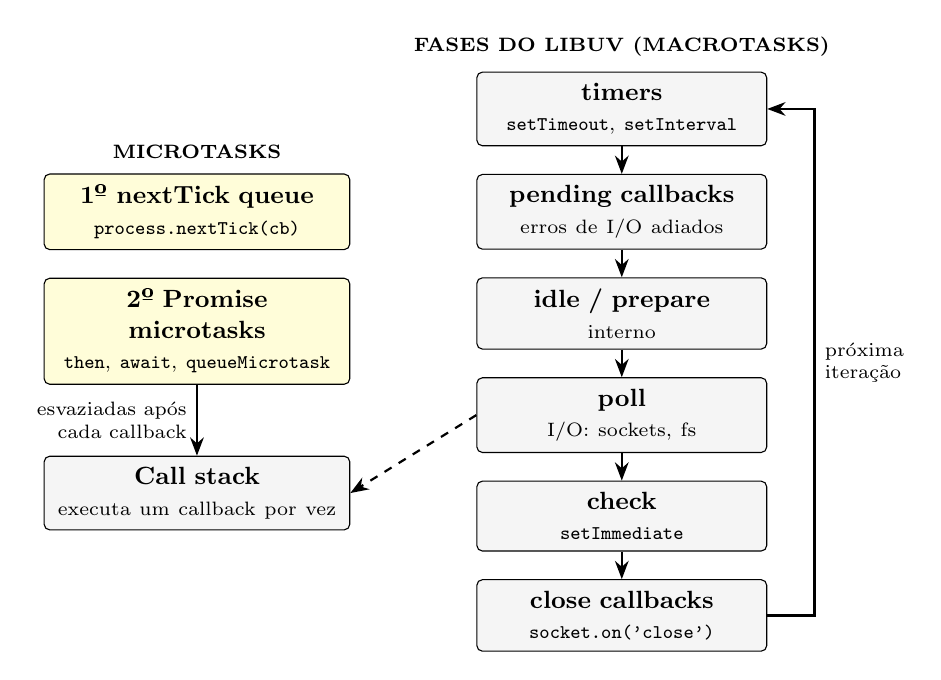
\begin{tikzpicture}[node distance=0.35cm, fase/.style={caixa=3.4cm}]
  \node[fase] (t) {\textbf{timers}\\\scriptsize\texttt{setTimeout}, \texttt{setInterval}};
  \node[fase, below=of t] (p) {\textbf{pending callbacks}\\\scriptsize erros de I/O adiados};
  \node[fase, below=of p] (i) {\textbf{idle / prepare}\\\scriptsize interno};
  \node[fase, below=of i] (po) {\textbf{poll}\\\scriptsize I/O: sockets, fs};
  \node[fase, below=of po] (ch) {\textbf{check}\\\scriptsize\texttt{setImmediate}};
  \node[fase, below=of ch] (cl) {\textbf{close callbacks}\\\scriptsize\texttt{socket.on('close')}};
  \draw[seta] (t) -- (p); \draw[seta] (p) -- (i); \draw[seta] (i) -- (po); \draw[seta] (po) -- (ch); \draw[seta] (ch) -- (cl);
  \draw[seta] (cl.east) -- ++(0.6,0) |- node[pos=0.25, right, font=\scriptsize, align=left]{próxima\\iteração} (t.east);
  \node[caixa=3.6cm, left=1.6cm of p, fill=yellow!15] (nt) {\textbf{1º nextTick queue}\\\scriptsize\texttt{process.nextTick(cb)}};
  \node[caixa=3.6cm, below=of nt, fill=yellow!15] (pr) {\textbf{2º Promise microtasks}\\\scriptsize\texttt{then}, \texttt{await}, \texttt{queueMicrotask}};
  \node[caixa=3.6cm, below=0.9cm of pr] (stack) {\textbf{Call stack}\\\scriptsize executa um callback por vez};
  \node[above=2pt of nt, font=\scriptsize\bfseries] {MICROTASKS};
  \node[above=2pt of t, font=\scriptsize\bfseries] {FASES DO LIBUV (MACROTASKS)};
  \draw[seta] (pr) -- node[left, font=\scriptsize, align=right]{esvaziadas após\\cada callback} (stack);
  \draw[seta, dashed] (po.west) -- (stack.east);
\end{tikzpicture}
\caption{Uma iteração do Event Loop no Node.js. Entre cada callback, o Node esvazia a fila de \texttt{nextTick} e depois a de Promises. Operações de \texttt{fs}, \texttt{dns.lookup}, \texttt{crypto} e \texttt{zlib} usam o thread pool do libuv (4 threads por padrão).}
\end{figure}

Preveja a saída antes de ler os comentários:

\begin{minted}{javascript}
console.log('A: síncrono');
setTimeout(() => console.log('E: timeout'), 0);
setImmediate(() => console.log('F: immediate'));
Promise.resolve().then(() => console.log('D: promise'));
process.nextTick(() => console.log('C: nextTick'));
console.log('B: síncrono');

// CommonJS: A, B, C, D e depois E/F em ordem NÃO garantida no módulo principal.
// Dentro de um callback de I/O, setImmediate sempre roda antes de setTimeout(0).
// ESM: o módulo é avaliado de forma assíncrona, então D costuma sair antes de C.
\end{minted}

\begin{cuidado}[Por que isso importa em produção]
Um \code{JSON.parse} de 50~MB, um loop pesado ou \code{crypto.pbkdf2Sync} bloqueiam a call stack: nenhuma outra requisição é atendida enquanto isso roda. Um \code{nextTick} recursivo pode deixar o I/O sem vez (\emph{starvation}).
\end{cuidado}

\dom{você prevê a ordem de logs mistos, explica a diferença entre micro e macrotasks e entre \code{nextTick} e \code{setImmediate}, e diagnostica ``o servidor travou'' como bloqueio do Event Loop.}

\section{Prototype}
\label{sec:prototype}
\index{prototype chain}
\alta

Todo objeto tem um link interno \code{[[Prototype]]}. Ao acessar uma propriedade que o objeto não tem, o JS sobe por essa cadeia. \code{class} é açúcar sintático sobre esse mecanismo: os métodos ficam no \code{prototype} do construtor, não em cada instância. \code{prototype} é a propriedade das \emph{funções construtoras}; \code{\_\_proto\_\_} é o acessor legado do link de \emph{qualquer objeto} --- prefira \code{Object.getPrototypeOf}.

\begin{figure}[h]
\centering
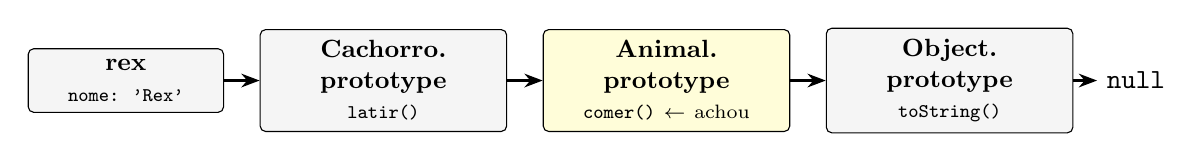
\begin{tikzpicture}[node distance=0.45cm]
  \node[caixa=2.2cm] (rex) {\textbf{rex}\\\scriptsize\texttt{nome: 'Rex'}};
  \node[caixa=2.85cm, right=of rex] (cp) {\textbf{Cachorro.}\\\textbf{prototype}\\\scriptsize\texttt{latir()}};
  \node[caixa=2.85cm, right=of cp, fill=yellow!15] (ap) {\textbf{Animal.}\\\textbf{prototype}\\\scriptsize\texttt{comer()} $\leftarrow$ achou};
  \node[caixa=2.85cm, right=of ap] (op) {\textbf{Object.}\\\textbf{prototype}\\\scriptsize\texttt{toString()}};
  \node[right=0.3cm of op] (n) {\texttt{null}};
  \draw[seta] (rex) -- (cp); \draw[seta] (cp) -- (ap); \draw[seta] (ap) -- (op); \draw[seta] (op) -- (n);
\end{tikzpicture}
\caption{Prototype chain. Cada seta é um \texttt{[[Prototype]]}. \texttt{rex.comer()} não está em \texttt{rex} nem em \texttt{Cachorro.prototype}; é encontrado em \texttt{Animal.prototype}.}
\end{figure}

\begin{minted}{javascript}
class Animal   { comer() { return 'comendo'; } }
class Cachorro extends Animal { latir() { return 'au'; } }
const rex = new Cachorro();

Object.getPrototypeOf(rex) === Cachorro.prototype;              // true
Object.getPrototypeOf(Cachorro.prototype) === Animal.prototype; // true
Object.hasOwn(rex, 'latir');   // false -- está no prototype
rex instanceof Animal;         // true -- percorre a cadeia
typeof Cachorro;               // 'function'
\end{minted}

\begin{nota}[Conexão com TypeScript]
\code{instanceof} faz narrowing porque é uma checagem de runtime real. Uma \code{interface} não existe em runtime: \code{x instanceof MinhaInterface} é erro de compilação. Por isso o TS usa tipagem estrutural (Seção~\ref{sec:structural}).
\end{nota}

\dom{você desenha a prototype chain de uma hierarquia de classes, sabe onde os métodos realmente vivem e explica por que \code{instanceof} falha quando existem duas cópias do mesmo pacote em \code{node\_modules}.}

\section{Prioridade média}
\label{sec:jsmedia}
\media

Você vai usar estes tópicos com frequência, mas eles não bloqueiam o entendimento do TypeScript.

\subsection{Map, Set, WeakMap e WeakSet}

{\small
\begin{tabularx}{\textwidth}{@{}llllX@{}}
\toprule
\textbf{Estrutura} & \textbf{Chaves} & \textbf{Referência} & \textbf{Iterável} & \textbf{Quando usar} \\
\midrule
\code{Map} & qualquer valor & forte & sim & dicionário dinâmico, cache \\
\code{Set} & valores únicos & forte & sim & deduplicação, ``já processado?'' \\
\code{WeakMap} & só objetos & fraca & não & metadados por objeto sem vazar memória \\
\code{WeakSet} & só objetos & fraca & não & marcar objetos visitados \\
\bottomrule
\end{tabularx}
}

\begin{minted}{typescript}
const cache = new Map<string, Promise<Usuario>>();   // id -> Promise em andamento
const vistos = new Set<string>();
const metadados = new WeakMap<object, { criadoEm: number }>(); // some com o objeto
const unicos = [...new Set(['a', 'b', 'a'])];       // ['a', 'b']
\end{minted}

\subsection{ESM e CommonJS}
\index{ESM}\index{CommonJS}

{\small
\begin{tabularx}{\textwidth}{@{}lXX@{}}
\toprule
 & \textbf{ESM} & \textbf{CommonJS} \\
\midrule
Sintaxe & \code{import} / \code{export} & \code{require} / \code{module.exports} \\
Carregamento & estático, analisado antes de executar; top-level \code{await} & dinâmico e síncrono \\
Exports & live bindings & o valor de \code{module.exports} no momento do require \\
Ativação no Node & \code{.mjs} ou \code{"type": "module"} & \code{.cjs} ou padrão \\
Imports relativos & extensão obrigatória (\code{./x.js}) & extensão opcional \\
Import dinâmico & \code{await import('./x.js')} & \code{require()} ou \code{import()} \\
\bottomrule
\end{tabularx}
}

Circular dependencies em CommonJS:

\begin{minted}{javascript}
// a.js
exports.pronto = false;
const b = require('./b');   // b.js roda AGORA e vê a pela metade
exports.pronto = true;

// b.js
const a = require('./a');   // recebe o exports PARCIAL de a
console.log(a.pronto);      // false
// Em ESM, acessar um binding ainda não inicializado lança ReferenceError (TDZ).
// Nos dois casos, o ciclo é um problema de design.
\end{minted}

\subsection{Outros tópicos de prioridade média}

{\small
\begin{tabularx}{\textwidth}{@{}lX@{}}
\toprule
\textbf{Tópico} & \textbf{O que dominar} \\
\midrule
\code{Symbol}, iterables, iterators & \code{Symbol.iterator} é o que faz \code{for...of} e spread funcionarem \\
\code{Intl} & formatação de número, moeda e data por locale \\
JSON & \code{parse} com \code{reviver}, \code{stringify} com \code{replacer}; o que não serializa (\code{Date}, \code{BigInt}, \code{undefined}) \\
Números & precisão de float, \code{BigInt}, \code{Number.isNaN}, \code{Number.isFinite} \\
Datas & \code{Date} básico, UTC $\times$ local, ISO 8601 \\
Regex & o suficiente para validação e parsing simples \\
\bottomrule
\end{tabularx}
}

\begin{minted}{javascript}
0.1 + 0.2 === 0.3;              // false -- float IEEE 754; dinheiro em centavos inteiros
2n ** 64n;                      // 18446744073709551616n (BigInt)
Number.isNaN('abc');            // false  (o isNaN global faz coerção e retorna true)

new Intl.NumberFormat('pt-BR', { style: 'currency', currency: 'BRL' }).format(1234.5);
// 'R$ 1.234,50'

JSON.stringify({ id: 1n }, (_, v) => (typeof v === 'bigint' ? v.toString() : v));
JSON.parse(texto, (chave, v) => (chave === 'criadoEm' ? new Date(v) : v)); // reviver

const { default: plugin } = await import(`./plugins/${nome}.js`);  // import dinâmico
\end{minted}

\dom{você prefere \code{Map} a objeto literal para chaves dinâmicas, configura um projeto ESM com TypeScript do zero, entende \code{ERR\_REQUIRE\_ESM}, quebra ciclos de dependência e nunca representa dinheiro com float.}

\section{Prioridade baixa}
\label{sec:jsbaixa}
\baixa

São úteis, mas não devem consumir tempo no início. Saiba que existem e volte quando um problema concreto pedir.

{\small
\begin{tabularx}{\textwidth}{@{}lXX@{}}
\toprule
\textbf{Tópico} & \textbf{O mínimo para agora} & \textbf{Quando voltar} \\
\midrule
Generators & \code{function*} e \code{yield} pausam uma função & paginação preguiçosa, pipelines \\
Proxy e Reflect & interceptam operações em objetos & ORMs, validação, \code{reflect-metadata} \\
Coercion avançada & use \code{===}; conheça truthy/falsy & quase nunca; o TS barra a maioria \\
Quirks históricos & \code{typeof null === 'object'}, ASI & curiosidade, entrevistas \\
\code{with}, \code{eval} & existem; não use & nunca, em código de produção \\
\code{Symbol.toPrimitive}, \code{Symbol.hasInstance} & customizam coerção e \code{instanceof} & metaprogramação em bibliotecas \\
APIs de browser & DOM, \code{window}, \code{localStorage} & só se for trabalhar com front-end \\
\bottomrule
\end{tabularx}
}

\begin{nota}[Regra de corte]
Se o tópico não explica por que um código TypeScript se comporta de certo jeito em runtime e não aparece no seu trabalho atual, ele é prioridade baixa. Anote e siga.
\end{nota}

% =====================================================================
\chapter{TypeScript --- núcleo principal}
\label{cap:tsnucleo}

A maior parte do seu tempo vai para este capítulo. A progressão vai de \emph{descrever valores} a \emph{derivar tipos de outros tipos}.

{\small
\begin{tabularx}{\textwidth}{@{}lXl@{}}
\toprule
\textbf{Bloco} & \textbf{Você passa a conseguir\ldots} & \textbf{Prioridade} \\
\midrule
Fundamentos & descrever os dados do domínio & \Ta \\
Classes em TypeScript & modelar serviços, entidades e decorators & \Ta \\
Narrowing & trabalhar com unions com segurança & \Ta \\
Generics & escrever código reutilizável sem perder tipos & \Ta \\
Utility Types & derivar DTOs sem duplicar & \Ta \\
\code{keyof}, \code{typeof}, indexed access & extrair tipos de valores & \Ta \\
Mapped Types & transformar todas as chaves de um tipo & \Ta \\
Conditional Types & escolher tipos por condição & \Ta \\
\code{infer} & extrair partes de tipos & \Ta \\
Template Literal Types & tipar strings estruturadas & \Tm \\
\code{satisfies} & validar sem perder inferência & \Ta \\
\code{unknown}, \code{any}, \code{never} & lidar com dados externos e exaustividade & \Ta \\
Type Assertions & saber quando (não) mentir ao compilador & \Tm \\
Function Overloads & tipar funções com várias formas & \Tm \\
\bottomrule
\end{tabularx}
}

\section{Fundamentos}
\label{sec:tsfund}
\alta

Tipos primitivos, arrays e tuples (inclusive \code{readonly}), enums, union e intersection types, literal types, aliases, interfaces, \code{as const} e \code{import type}. Repare na \textbf{inferência}: você raramente precisa anotar variáveis locais.

\begin{minted}{typescript}
let id: number = 1;
const nome = 'ana';            // tipo literal 'ana' (const não muda)
let status = 'ativo';          // string -- let "alarga" o tipo (widening)
const ids: readonly number[] = [1, 2];                     // sem push/splice
const par: readonly [chave: string, valor: number] = ['idade', 30];

type Status = 'ativo' | 'inativo' | 'banido';               // union de literais
type ComId = { id: string };
type ComDatas = { criadoEm: Date; atualizadoEm: Date };
type Entidade = ComId & ComDatas;                           // intersection

interface Usuario {
  id: string;
  email: string;
  apelido?: string;           // opcional
  readonly criadoEm: Date;    // não pode ser reatribuído (em compile time)
  status: Status;
}

const ROTAS = { home: '/', pedidos: '/pedidos' } as const;  // literais + readonly
import type { Pedido } from './pedido.js';                  // apagado no emit
\end{minted}

\code{enum}, \code{const enum} ou union literal?

\begin{minted}{typescript}
enum Papel { Admin, Leitor }        // gera objeto em runtime; Papel[0] === 'Admin'
const enum Cor { Azul, Verde }      // inlined no emit; problemático com isolatedModules

const PAPEL = { Admin: 'admin', Leitor: 'leitor' } as const;
type Papel2 = (typeof PAPEL)[keyof typeof PAPEL];   // 'admin' | 'leitor' -- recomendado
\end{minted}

\begin{center}
\begin{tabular}{@{}lll@{}}
\toprule
\textbf{Aspecto} & \code{interface} & \code{type} \\
\midrule
Objetos & sim & sim \\
Unions, tuples, primitivos & não & sim \\
Intersections & via \code{extends} & sim (\code{\&}) \\
Declaration merging & sim & não \\
Extensível por terceiros & sim & não \\
Mapped / conditional & não & sim \\
Uso recomendado & contratos de objeto & composições e unions \\
\bottomrule
\end{tabular}
\end{center}

\dom{você modela um agregado de domínio (\code{Pedido} com itens, status e pagamento) sem \code{any}, prefere union literal a \code{enum} e explica por que \code{let x = 'a'} vira \code{string} enquanto \code{const x = 'a'} vira \code{'a'}.}

\section{Classes em TypeScript}
\label{sec:classes}
\index{decorators}
\alta

\begin{itemize}
  \item \code{public}, \code{private}, \code{protected}, \code{readonly} e parameter properties;
  \item classes e métodos \code{abstract}, \code{override}, \code{implements};
  \item \code{this} types (métodos encadeáveis);
  \item decorators de classe, método e propriedade, e metadata reflection (base do NestJS, TypeORM e class-validator).
\end{itemize}

\begin{minted}{typescript}
interface Repositorio<T> {
  buscar(id: string): Promise<T | undefined>;
}

abstract class RepositorioBase<T extends { id: string }> implements Repositorio<T> {
  protected readonly itens = new Map<string, T>();
  abstract nomeTabela(): string;

  async buscar(id: string) { return this.itens.get(id); }
  salvar(item: T): this {                // 'this' type: subclasses mantêm o tipo
    this.itens.set(item.id, item);
    return this;
  }
}

class RepositorioPedidos extends RepositorioBase<Pedido> {
  constructor(private readonly db: Db) { super(); }  // parameter property
  override nomeTabela() { return 'pedidos'; }       // override explícito
}
\end{minted}

Decorators no padrão TC39 (TS 5.0+, sem \code{experimentalDecorators}):

\begin{minted}{typescript}
function log<This, Args extends unknown[], R>(
  alvo: (this: This, ...args: Args) => R,
  contexto: ClassMethodDecoratorContext<This, (this: This, ...args: Args) => R>,
) {
  return function (this: This, ...args: Args): R {
    console.log(`-> ${String(contexto.name)}`, args);
    return alvo.call(this, ...args);
  };
}

class ServicoPagamento {
  @log
  cobrar(valor: number) { return valor * 1.02; }
}
\end{minted}

\begin{cuidado}[Dois sistemas de decorators]
NestJS, TypeORM e class-validator usam os decorators \emph{legados} (\code{experimentalDecorators} + \code{emitDecoratorMetadata} + \code{reflect-metadata}), que incluem decorators de \emph{parâmetro} e emitem metadados de tipo em runtime. Os decorators TC39 não têm decorators de parâmetro nem emitem esses metadados. Saiba qual sistema o seu framework usa.
\end{cuidado}

\dom{você escreve uma hierarquia com \code{abstract}, \code{override} e parameter properties, implementa um decorator de método simples e explica o que \code{emitDecoratorMetadata} gera em runtime para a injeção de dependências do NestJS funcionar.}

\section{Narrowing}
\label{sec:narrowing}
\index{narrowing}
\alta

Narrowing é o TypeScript \textbf{acompanhando checagens de runtime} para estreitar um tipo dentro de um bloco. É onde TS e JS mais se encontram: todo narrowing se apoia em algo que realmente executa.

\begin{minted}{typescript}
function formatar(v: string | number | Date | null): string {
  if (v === null) return '-';                    // equality narrowing
  if (typeof v === 'string') return v.trim();    // typeof
  if (v instanceof Date) return v.toISOString(); // instanceof (prototype chain)
  return v.toFixed(2);                           // sobrou: number
}

type Peixe = { nadar(): void };
type Passaro = { voar(): void };
function mover(animal: Peixe | Passaro) {
  if ('nadar' in animal) animal.nadar();         // in
  else animal.voar();
}

function tamanho(s?: string) {
  if (!s) return 0;    // truthiness: cuidado, '' também cai aqui
  return s.length;
}
\end{minted}

Type predicates, assertion functions e discriminated unions\index{discriminated union}:

\begin{minted}{typescript}
type Resultado<T> =
  | { ok: true; valor: T }
  | { ok: false; erro: string };     // "ok" é o discriminante

function dobrar(r: Resultado<number>) {
  if (r.ok) return r.valor * 2;      // r: { ok: true; valor: number }
  return r.erro;                     // r: { ok: false; erro: string }
}

function isString(x: unknown): x is string {        // type predicate
  return typeof x === 'string';
}
const nomes = ['a', 1, 'b'].filter(isString);       // string[]
// TS 5.5+: .filter(x => typeof x === 'string') já infere o predicate

function assertDefinido<T>(v: T, msg: string): asserts v is NonNullable<T> {
  if (v === null || v === undefined) throw new Error(msg);  // assertion function
}
const url = process.env.DATABASE_URL;
assertDefinido(url, 'DATABASE_URL ausente');
url.startsWith('postgres');                         // url: string daqui em diante
\end{minted}

\dom{você modela estados (\code{pendente | pago | cancelado}) como discriminated union, escreve predicates e assertion functions corretos e sabe que um predicate errado engana o compilador.}

\section{Generics}
\label{sec:generics}
\index{generics}
\alta

Generics são \textbf{parâmetros de tipo}: permitem que uma função, interface ou classe preserve a relação entre entrada e saída. Constraints (\code{extends}) limitam o que o parâmetro aceita; defaults (\code{<T = unknown>}) definem o valor quando nada é informado.

\begin{minted}{typescript}
function primeiro<T>(itens: T[]): T | undefined {   // função genérica
  return itens[0];
}

interface Resposta<T = unknown, E = Error> {        // interface com defaults
  dados?: T;
  erro?: E;
}

class Cache<K, V> {                                 // classe genérica
  #mapa = new Map<K, V>();
  get(chave: K) { return this.#mapa.get(chave); }  // V | undefined
  set(chave: K, valor: V) { this.#mapa.set(chave, valor); return this; }
}

function maiorPor<T extends { length: number }>(a: T, b: T): T { // constraint
  return a.length >= b.length ? a : b;
}
\end{minted}

\code{keyof} e \code{T[K]} expressam a relação entre chave e valor:

\begin{minted}{typescript}
function atualizarCampo<T, K extends keyof T>(
  objeto: T,
  campo: K,
  valor: T[K]
): T {
  return {
    ...objeto,
    [campo]: valor
  };
}

const u = { nome: 'Ana', idade: 30 };
atualizarCampo(u, 'idade', 31);    // ok
atualizarCampo(u, 'idade', '31');  // erro: string não é atribuível a number
atualizarCampo(u, 'email', 'x');   // erro: 'email' não é keyof typeof u
\end{minted}

\begin{nota}[Heurística]
Se um parâmetro de tipo aparece uma única vez na assinatura, ele provavelmente não precisa existir: \code{function log<T>(x: T): void} é só \code{function log(x: unknown): void}. Generics servem para \textbf{relacionar} tipos.
\end{nota}

\dom{você escreve constraints sem consultar, cria um \code{Repository<T extends \{ id: string \}>} genérico, explica \code{K extends keyof T} e reconhece quando um generic é desnecessário.}

\section{Utility Types}
\label{sec:utility}
\index{utility types}
\alta

Tipos prontos da biblioteca padrão que transformam outros tipos. Todos são implementados com mapped e conditional types; depois da Seção~\ref{sec:infer} você consegue reescrever cada um.

{\small
\begin{tabularx}{\textwidth}{@{}lXX@{}}
\toprule
\textbf{Utility} & \textbf{O que faz} & \textbf{Uso no backend} \\
\midrule
\code{Partial<T>} & todas as propriedades opcionais & body de \code{PATCH} \\
\code{Required<T>} & todas obrigatórias & config após aplicar defaults \\
\code{Readonly<T>} & todas \code{readonly} (raso) & value objects \\
\code{Pick<T, K>} & mantém só as chaves \code{K} & resposta pública \\
\code{Omit<T, K>} & remove as chaves \code{K} & DTO de criação \\
\code{Record<K, V>} & objeto com chaves \code{K} e valores \code{V} & handler por tipo de evento \\
\code{Exclude<U, E>} & remove membros de uma union & \code{Exclude<Status, 'banido'>} \\
\code{Extract<U, E>} & mantém membros atribuíveis a \code{E} & subtipo de evento \\
\code{NonNullable<T>} & remove \code{null} e \code{undefined} & após validar presença \\
\code{ReturnType<F>} & tipo de retorno de uma função & tipo de uma factory \\
\code{Parameters<F>} & tupla dos parâmetros & wrappers e mocks \\
\code{ConstructorParameters<C>} & tupla dos parâmetros do construtor & factories de classes \\
\code{InstanceType<C>} & tipo da instância de uma classe & containers de DI \\
\code{Awaited<T>} & desembrulha Promise (recursivo) & resultado de função async \\
\code{ThisParameterType<F>} & tipo do parâmetro \code{this} & funções que dependem de contexto \\
\code{OmitThisParameter<F>} & remove o parâmetro \code{this} & após \code{bind} \\
\bottomrule
\end{tabularx}
}

\begin{minted}{typescript}
interface Usuario {
  id: string; email: string; senhaHash: string;
  nome: string; papel: 'admin' | 'leitor'; criadoEm: Date;
}

type CriarUsuarioDTO =
  Omit<Usuario, 'id' | 'criadoEm' | 'senhaHash'> & { senha: string };
type AtualizarUsuarioDTO = Partial<Omit<Usuario, 'id' | 'criadoEm'>>;
type UsuarioPublico = Readonly<Pick<Usuario, 'id' | 'nome' | 'papel'>>;
type HandlersPorPapel = Record<Usuario['papel'], (u: Usuario) => void>;

class Conexao { constructor(host: string, porta: number) {} }
type ArgsConexao = ConstructorParameters<typeof Conexao>; // [host: string, porta: number]
type Instancia   = InstanceType<typeof Conexao>;          // Conexao

function formatar(this: { moeda: string }, v: number) { return `${this.moeda} ${v}`; }
type Contexto = ThisParameterType<typeof formatar>;       // { moeda: string }
type Solta    = OmitThisParameter<typeof formatar>;       // (v: number) => string
\end{minted}

\dom{você deriva DTOs do tipo de domínio em vez de redeclarar campos e sabe a diferença entre \code{Omit} (chaves de objeto) e \code{Exclude} (membros de union).}

\section{\texttt{keyof}, \texttt{typeof} e indexed access}
\label{sec:keyof}
\alta

Três ferramentas para \textbf{derivar tipos}: \code{typeof} (em posição de tipo) extrai o tipo de um \emph{valor}; \code{keyof} extrai a union das chaves de um tipo; \code{T[K]} acessa o tipo de uma propriedade. Combinadas, fazem do valor a fonte da verdade.

\begin{minted}{typescript}
const config = { porta: 3000, host: 'localhost', debug: false };

type Config      = typeof config;         // { porta: number; host: string; ... }
type ChaveConfig = keyof Config;          // 'porta' | 'host' | 'debug'
type Porta       = Config['porta'];       // number
type Valores     = Config[keyof Config];  // number | string | boolean

const EVENTOS = ['criado', 'pago', 'cancelado'] as const;
type Evento = (typeof EVENTOS)[number];   // 'criado' | 'pago' | 'cancelado'

async function buscarUsuario(id: string) { return { id, nome: 'Ana' }; }
type UsuarioDb = Awaited<ReturnType<typeof buscarUsuario>>;
\end{minted}

\begin{center}
\begin{tabular}{@{}lll@{}}
\toprule
\textbf{Expressão} & \textbf{Onde existe} & \textbf{Resultado} \\
\midrule
\code{typeof x === 'string'} & runtime (JS) & uma string: \code{'string'}, \code{'object'}\ldots \\
\code{type T = typeof x} & compile time (TS) & o tipo estático de \code{x} \\
\code{keyof T} & compile time & union das chaves \\
\code{Object.keys(x)} & runtime & \code{string[]} \\
\bottomrule
\end{tabular}
\end{center}

\dom{você cria uma union a partir de um array \code{as const} e explica por que \code{Object.keys} retorna \code{string[]}, e não \code{(keyof T)[]}: a tipagem estrutural permite propriedades extras.}

\section{Mapped Types}
\label{sec:mapped}
\index{mapped types}
\alta

Um mapped type percorre as chaves de um tipo e produz um novo tipo --- um \code{for...in} em nível de tipo. Modificadores \code{+?}, \code{-?}, \code{+readonly} e \code{-readonly} adicionam ou removem opcionalidade e imutabilidade; a cláusula \code{as} renomeia ou filtra chaves.

\begin{minted}{typescript}
type Opcional<T> = {
  [K in keyof T]?: T[K];
};

type SomenteLeitura<T> = { +readonly [K in keyof T]: T[K] };
type Mutavel<T>        = { -readonly [K in keyof T]: T[K] };  // remove modificador
type Obrigatorio<T>    = { [K in keyof T]-?: T[K] };          // remove o '?'

type Validadores<T> = { [K in keyof T]: (valor: T[K]) => boolean };
const validarUsuario: Validadores<{ email: string; idade: number }> = {
  email: (v) => v.includes('@'),   // v: string
  idade: (v) => v >= 18,           // v: number
};

type SemFuncoes<T> = { [K in keyof T as T[K] extends Function ? never : K]: T[K] };
\end{minted}

\dom{você reescreve \code{Partial}, \code{Readonly} e \code{Record} de memória, usa key remapping com \code{as} e cria tipos como \code{Validadores<T>} para o seu domínio.}

\section{Conditional Types}
\label{sec:conditional}
\index{conditional types}\index{distributividade}
\alta

A forma \code{T extends U ? X : Y} significa: se \code{T} é atribuível a \code{U}, o resultado é \code{X}; senão, \code{Y}. Quando \code{T} é um parâmetro ``nu'' e recebe uma union, a condição é aplicada a \textbf{cada membro} (distributividade). Para evitar, envolva em tupla: \code{[T] extends [U]}.

\begin{minted}{typescript}
type EhString<T> = T extends string ? true : false;
type A = EhString<'x'>;   // true
type B = EhString<42>;    // false

type ParaArray<T> = T extends unknown ? T[] : never;
type C = ParaArray<string | number>;       // string[] | number[]  (distribui)

type ParaArrayJunto<T> = [T] extends [unknown] ? T[] : never;
type D = ParaArrayJunto<string | number>;  // (string | number)[]  (não distribui)

type MeuExclude<T, U> = T extends U ? never : T;  // é assim que Exclude funciona
type E = MeuExclude<'a' | 'b' | 'c', 'a'>;        // 'b' | 'c'
\end{minted}

\dom{você explica por que \code{Exclude} funciona (distributividade + \code{never} desaparece da union) e sabe desligar a distribuição com \code{[T]}.}

\section{\texttt{infer}}
\label{sec:infer}
\index{infer}
\alta

\code{infer} declara uma variável de tipo dentro de um conditional type, capturando uma parte da estrutura. Do simples ao avançado, incluindo conditional types aninhados e variadic tuples:

\begin{minted}{typescript}
// nível 1 -- elemento de um array
type Elemento<T> = T extends (infer E)[] ? E : never;
type N1 = Elemento<string[]>;                        // string

// nível 2 -- reimplementando ReturnType
type Retorno<F> = F extends (...args: any[]) => infer R ? R : never;
type N2 = Retorno<() => Promise<number>>;             // Promise<number>

// nível 3 -- desembrulhar Promise recursivamente (ideia do Awaited)
type Desembrulhar<T> = T extends Promise<infer V> ? Desembrulhar<V> : T;
type N3 = Desembrulhar<Promise<Promise<number>>>;     // number

// nível 4 -- cabeça e cauda de tupla (variadic)
type Cabeca<T extends unknown[]> = T extends [infer H, ...unknown[]] ? H : never;
type Cauda<T extends unknown[]>  = T extends [unknown, ...infer R] ? R : [];
type N4 = Cauda<[string, number, boolean]>;           // [number, boolean]

// nível 5 -- infer em template literal: parâmetros de rota
type ParamsRota<S extends string> =
  S extends `${string}:${infer P}/${infer Resto}`
    ? P | ParamsRota<`/${Resto}`>
    : S extends `${string}:${infer P}` ? P : never;

type N5 = ParamsRota<'/usuarios/:id/pedidos/:pedidoId'>; // 'id' | 'pedidoId'
\end{minted}

\dom{você implementa versões simplificadas de \code{ReturnType}, \code{Parameters} e \code{Awaited} e lê o tipo do nível 5 explicando cada passo da recursão.}

\section{Template Literal Types}
\label{sec:template}
\index{template literal types}
\media

A mesma sintaxe das template strings, em nível de tipo. Combinadas com unions, geram todas as combinações; com mapped types (cláusula \code{as}), renomeiam chaves. Os intrínsecos \code{Uppercase}, \code{Lowercase}, \code{Capitalize} e \code{Uncapitalize} transformam literais.

\begin{minted}{typescript}
type Metodo  = 'GET' | 'POST' | 'DELETE';
type Recurso = 'usuarios' | 'pedidos';
type Permissao = `${Lowercase<Metodo>}:${Recurso}`;
// 'get:usuarios' | 'get:pedidos' | 'post:usuarios' | ... (6 combinações)

type Eventos<T> = {
  [K in keyof T & string as `on${Capitalize<K>}Alterado`]: (novo: T[K]) => void;
};

// Path<T>: todos os caminhos com ponto de um objeto aninhado
type Path<T> = T extends object
  ? { [K in keyof T & string]: T[K] extends object ? K | `${K}.${Path<T[K]>}` : K }[keyof T & string]
  : never;

type Config = { db: { host: string; porta: number }; debug: boolean };
type Caminhos = Path<Config>;   // 'db' | 'db.host' | 'db.porta' | 'debug'
\end{minted}

\dom{você tipa chaves de cache, nomes de eventos, permissões ou caminhos de configuração com template literal types e usa \code{Capitalize}/\code{Uppercase} em key remapping.}

\section{\texttt{satisfies}}
\label{sec:satisfies}
\index{satisfies}
\alta

Uma \textbf{anotação} (\code{const x: T = \ldots}) substitui o tipo inferido por \code{T} e alarga os literais. O operador \code{satisfies} (TS 4.9+) \textbf{verifica} se o valor é compatível com \code{T}, mas mantém o tipo inferido, mais preciso.

\begin{minted}{typescript}
// anotação: tipo declarado, literais alargados
const config: Record<string, string> = { host: 'localhost' };
config.host;        // string
config.naoExiste;   // compila: qualquer string é chave válida

// satisfies: valida a forma e preserva o tipo inferido
const config2 = { host: 'localhost' } satisfies Record<string, string>;
config2.host;       // string (chave conhecida)
config2.naoExiste;  // erro: a chave não existe

const config3 = { host: 'localhost' } as const satisfies Record<string, string>;
config3.host;       // 'localhost' -- o literal, readonly

type Cor = string | [number, number, number];
const paleta = { primaria: [49, 120, 198], fundo: '#0b0f17' } satisfies Record<string, Cor>;
paleta.fundo.toUpperCase();   // ok: o TS lembra que é string, não Cor
paleta.primaria[0];           // number -- tupla preservada
\end{minted}

\begin{center}
\begin{tabular}{@{}llll@{}}
\toprule
 & \textbf{Anotação \code{: T}} & \textbf{\code{satisfies T}} & \textbf{\code{as T}} \\
\midrule
Verifica compatibilidade & sim & sim & quase nada \\
Tipo resultante & \code{T} (alargado) & o inferido & \code{T} \\
Checa propriedades extras & sim & sim & não \\
Uso ideal & contratos, parâmetros & configs, mapas, rotas & raramente \\
\bottomrule
\end{tabular}
\end{center}

\dom{você usa \code{as const satisfies} em tabelas de configuração e rotas e explica em uma frase quando preferir \code{satisfies}, anotação ou \code{as const}.}

\section{\texttt{unknown}, \texttt{any} e \texttt{never}}
\label{sec:unknown}
\index{unknown}\index{never}
\alta

{\small
\begin{tabularx}{\textwidth}{@{}lXXX@{}}
\toprule
\textbf{Tipo} & \textbf{Significa} & \textbf{Pode usar direto?} & \textbf{Quando usar} \\
\midrule
\code{any} & desliga a checagem & sim --- e contamina o resto & quase nunca; migração de JS \\
\code{unknown} & o ``any seguro'' & não: precisa de narrowing & dados externos: JSON, body, \code{catch} \\
\code{never} & ``não pode existir'' & --- & exhaustive checks, funções que sempre lançam \\
\bottomrule
\end{tabularx}
}

\begin{minted}{typescript}
function lerJson(texto: string): unknown {
  return JSON.parse(texto);        // JSON.parse retorna any; "fechamos" em unknown
}
const dado = lerJson(body);
dado.nome;                         // erro: 'dado' is of type 'unknown'
if (typeof dado === 'object' && dado !== null && 'nome' in dado) {
  dado.nome;                       // ok, depois de provar
}

try { await pagar(); } catch (err) {  // err: unknown (strict)
  const msg = err instanceof Error ? err.message : String(err);
}
\end{minted}

Exhaustive check com \code{never}:

\begin{minted}{typescript}
function assertNever(x: never): never {
  throw new Error(`Caso não tratado: ${JSON.stringify(x)}`);
}

type Pagamento =
  | { tipo: 'pix'; chave: string }
  | { tipo: 'cartao'; bandeira: string }
  | { tipo: 'boleto'; vencimento: Date };

function taxa(p: Pagamento): number {
  switch (p.tipo) {
    case 'pix':    return 0;
    case 'cartao': return 0.03;
    case 'boleto': return 2.5;
    default:       return assertNever(p);  // novo tipo na union? erro AQUI
  }
}
\end{minted}

\dom{seu código de fronteira (HTTP, filas, variáveis de ambiente) recebe \code{unknown} e valida; você usa \code{assertNever} para que um caso novo quebre a compilação em todo \code{switch} esquecido.}

\section{Type Assertions}
\label{sec:assertions}
\media

\code{as} e a non-null assertion \code{!} não convertem nem checam nada em runtime: eles \textbf{mandam o compilador acreditar em você}.

\begin{minted}{typescript}
const usuario = corpo as Usuario;        // nenhuma validação acontece
const porta = process.env.PORT!;         // "não é undefined" -- e se for?
const n = 'texto' as unknown as number;  // double assertion: alarme vermelho
const rotas = ['/a', '/b'] as const;     // as const: outra coisa, congela literais

// melhor: prove em runtime e deixe o narrowing trabalhar
const portaSegura = Number(process.env.PORT ?? 3000);
\end{minted}

\textbf{Quando é aceitável:} depois de uma validação que o compilador não consegue acompanhar; em testes (mocks parciais); ao contornar uma biblioteca mal tipada. Para configurações, \code{satisfies} é a alternativa segura.

\textbf{Riscos:} esconde bugs até a produção e sobrevive a refatorações sem avisar. Usar \code{!} em \code{Map.get}, \code{find} e variáveis de ambiente é a origem clássica de \code{Cannot read properties of undefined}.

\dom{você justifica cada \code{as} e \code{!} do seu código e troca a maioria por narrowing, \code{satisfies} ou validação de schema.}

\section{Function Overloads}
\label{sec:overloads}
\media

Overloads declaram várias assinaturas para uma única implementação. Use quando o \textbf{tipo de retorno depende do tipo do argumento} de um jeito que uma union não expressa.

\begin{minted}{typescript}
function buscar(id: string): Promise<Usuario>;
function buscar(ids: string[]): Promise<Usuario[]>;
function buscar(arg: string | string[]): Promise<Usuario | Usuario[]> {
  return Array.isArray(arg) ? repo.buscarVarios(arg) : repo.buscarUm(arg);
}
const um     = await buscar('u1');          // Usuario
const varios = await buscar(['u1', 'u2']);  // Usuario[]

// quando o retorno NÃO depende da entrada, uma union basta:
function registrar(erro: string | Error): void { /* ... */ }
\end{minted}

\begin{cuidado}
A assinatura de implementação não é visível para quem chama, e o TS não verifica se a implementação respeita cada overload. Se der para resolver com union ou com generic + conditional type, prefira.
\end{cuidado}

\dom{você decide entre union, generic e overload olhando apenas para a relação entrada $\rightarrow$ saída.}

% =====================================================================
\chapter{TypeScript avançado}
\label{cap:tsavancado}

O que separa quem usa TypeScript de quem projeta com TypeScript.

{\small
\begin{tabularx}{\textwidth}{@{}lXl@{}}
\toprule
\textbf{Tópico} & \textbf{Resumo} & \textbf{Prioridade} \\
\midrule
Structural typing & compatibilidade pela forma, não pelo nome & \Ta \\
Configuração do \code{tsconfig} & as flags definem quão seguro é o projeto & \Ta \\
Variance & co-, contra-, bi- e invariância & \Tm \\
Tipos recursivos & JSON, árvores, \code{DeepPartial} & \Tm \\
Branded / opaque types & IDs que não se misturam & \Tm \\
Variadic tuple types & manipular listas de argumentos & \Tm \\
Declaration files \code{.d.ts} & próprios, \code{@types/*}, ambientes e globais & \Tm \\
Module augmentation & estender tipos de bibliotecas & \Tm \\
Tipos de bibliotecas externas & \code{@types}, \code{exports}, \code{skipLibCheck} & \Tm \\
Conditional e mapped complexos & filtrar chaves, gerar APIs tipadas & \Tb \\
Declaration merging e \code{namespace} & fusão de declarações; namespace é legado & \Tb \\
Inferência avançada & \code{const} type parameters, \code{NoInfer} & \Tb \\
Type-level programming & recursão com acumuladores & \Tb \\
\bottomrule
\end{tabularx}
}

\section{Structural Typing}
\label{sec:structural}
\index{structural typing}
\alta

Um tipo é compatível com outro se tiver \textbf{a forma exigida}; o nome da classe ou interface é irrelevante. Isso espelha o \emph{duck typing} do JavaScript, onde interfaces não existem em runtime. Linguagens como Java e C\# usam \emph{nominal typing}: dois tipos com a mesma forma, mas nomes diferentes, são incompatíveis.

\begin{figure}[h]
\centering
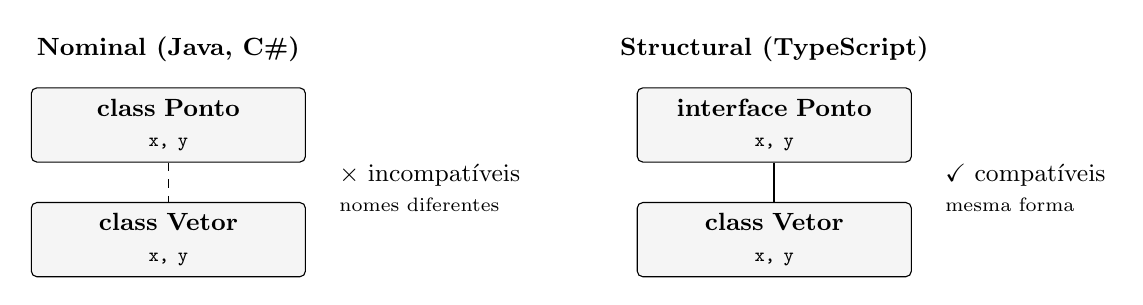
\begin{tikzpicture}[node distance=0.5cm]
  \node[caixa=3.2cm] (np) {\textbf{class Ponto}\\\scriptsize\texttt{x, y}};
  \node[caixa=3.2cm, below=of np] (nv) {\textbf{class Vetor}\\\scriptsize\texttt{x, y}};
  \node[font=\small, right=0.3cm of np, yshift=-0.8cm, align=left] (nr) {$\times$ incompatíveis\\\scriptsize nomes diferentes};
  \node[font=\small\bfseries, above=0.2cm of np] {Nominal (Java, C\#)};
  \node[caixa=3.2cm, right=4.2cm of np] (sp) {\textbf{interface Ponto}\\\scriptsize\texttt{x, y}};
  \node[caixa=3.2cm, below=of sp] (sv) {\textbf{class Vetor}\\\scriptsize\texttt{x, y}};
  \node[font=\small, right=0.3cm of sp, yshift=-0.8cm, align=left] (sr) {\checkmark\ compatíveis\\\scriptsize mesma forma};
  \node[font=\small\bfseries, above=0.2cm of sp] {Structural (TypeScript)};
  \draw[dashed] (np) -- (nv);
  \draw[thick] (sp) -- (sv);
\end{tikzpicture}
\caption{Nominal typing compara nomes; structural typing compara formas.}
\end{figure}

\begin{minted}{typescript}
interface Ponto { x: number; y: number }
class Pixel { constructor(public x: number, public y: number, public cor: string) {} }

const p: Ponto = new Pixel(1, 2, 'red');     // ok: tem x e y
const q: Ponto = { x: 1, y: 2, cor: 'red' }; // erro: excess property check
const tmp = { x: 1, y: 2, cor: 'red' };
const r: Ponto = tmp;                        // ok: a checagem extra só vale para literais
\end{minted}

\section{Variance}
\index{variance}
\media

{\small
\begin{tabularx}{\textwidth}{@{}lXX@{}}
\toprule
\textbf{Variância} & \textbf{Significa} & \textbf{Onde aparece} \\
\midrule
Covariância & \code{F<Sub>} é atribuível a \code{F<Super>} & retornos, arrays readonly \\
Contravariância & \code{F<Super>} é atribuível a \code{F<Sub>} & parâmetros de função \\
Bivariância & as duas direções são aceitas & parâmetros de \emph{métodos} (unsound) \\
Invariância & nenhuma direção & tipos lidos e escritos (\code{in out T}) \\
\bottomrule
\end{tabularx}
}

\begin{minted}{typescript}
class Animal { comer() {} }
class Cachorro extends Animal { latir() {} }

let animais: Animal[] = [];
let caes: Cachorro[] = [];
animais = caes;      // ok: arrays são covariantes (unsound: animais.push(new Animal()))

type Handler<T> = (valor: T) => void;
let hAnimal: Handler<Animal> = (a) => a.comer();
let hCao: Handler<Cachorro> = (c) => c.latir();
hCao = hAnimal;      // ok: parâmetros são contravariantes
hAnimal = hCao;      // erro com strictFunctionTypes: chamaria latir() num Animal

interface Caixa<in out T> { valor: T }  // variance annotation explícita (TS 4.7+)
\end{minted}

Métodos declarados com sintaxe de método (\code{m(x: T): void}) continuam bivariantes mesmo com \code{strictFunctionTypes}; propriedades do tipo função (\code{m: (x: T) => void}) são checadas.

\section{Tipos recursivos, variadic tuples e type-level programming}
\media

\begin{minted}{typescript}
type Json = string | number | boolean | null | Json[] | { [chave: string]: Json };

type DeepPartial<T> = {
  [K in keyof T]?: T[K] extends object ? DeepPartial<T[K]> : T[K];
};

// chaves cujo valor é de um certo tipo
type ChavesDoTipo<T, V> = { [K in keyof T]: T[K] extends V ? K : never }[keyof T];

// variadic tuple types
type Concat<A extends unknown[], B extends unknown[]> = [...A, ...B];
type R = Concat<[string], [number, boolean]>;   // [string, number, boolean]

function comContexto<A extends unknown[], T>(fn: (ctx: Contexto, ...args: A) => T) {
  return (...args: A) => fn(contextoAtual(), ...args);  // remove o 1º parâmetro
}

// type-level programming: recursão com acumulador
type Tupla<N extends number, Acc extends unknown[] = []> =
  Acc['length'] extends N ? Acc : Tupla<N, [...Acc, unknown]>;
type Soma<A extends number, B extends number> = [...Tupla<A>, ...Tupla<B>]['length'];
type Cinco = Soma<2, 3>;   // 5
\end{minted}

\begin{cuidado}[Use com moderação]
Tipos complexos têm custo: mensagens de erro ilegíveis, compilação mais lenta e colegas que não conseguem manter o código. Programação em nível de tipo compensa em bibliotecas; em código de aplicação, prefira tipos simples e explícitos.
\end{cuidado}

\section{Branded Types}
\index{branded types}
\media

Como a tipagem é estrutural, \code{UsuarioId} e \code{PedidoId} declarados como \code{string} se misturam. Um \emph{brand} (ou \emph{opaque type}) adiciona uma propriedade fantasma que só existe em compile time, simulando tipagem nominal.

\begin{minted}{typescript}
type Brand<T, B extends string> = T & { readonly __brand: B };
type UsuarioId = Brand<string, 'UsuarioId'>;
type PedidoId  = Brand<string, 'PedidoId'>;

function paraUsuarioId(v: string): UsuarioId {  // "smart constructor": valide aqui
  if (!v.startsWith('usr_')) throw new Error('id inválido');
  return v as UsuarioId;                        // a única assertion, num só lugar
}

declare function buscarPedido(id: PedidoId): Promise<unknown>;
const uid = paraUsuarioId('usr_42');
buscarPedido(uid);  // erro: UsuarioId não é PedidoId -- mesmo sendo string em runtime
\end{minted}

\section{Declaration files, module augmentation e declaration merging}
\index{module augmentation}\index{declaration merging}
\media

Três conceitos que costumam ser confundidos:

\begin{itemize}
  \item \textbf{Declaration file (\code{.d.ts})}: só declarações, sem implementação. Pode ser seu, vir de \code{@types/*}, declarar um \emph{módulo ambiente} (\code{declare module 'x'}) ou globais ambientes (\code{declare global}).
  \item \textbf{Declaration merging}: duas declarações com o mesmo nome se fundem (duas \code{interface Foo}, ou \code{namespace} + função).
  \item \textbf{Module augmentation}: usar declaration merging para \emph{estender um módulo existente} a partir de outro arquivo.
\end{itemize}

\begin{minted}{typescript}
// types/lib-legada.d.ts -- módulo ambiente para uma lib JS sem tipos
declare module 'lib-legada' {
  export function calcular(valor: number, taxa?: number): number;
  export const versao: string;
}
\end{minted}

\begin{minted}{typescript}
// env.d.ts -- global ambiente
declare global {
  namespace NodeJS {
    interface ProcessEnv {
      DATABASE_URL: string;
      NODE_ENV: 'development' | 'production' | 'test';
    }
  }
}
export {};
\end{minted}

\begin{minted}{typescript}
// fastify.d.ts -- module augmentation
import 'fastify';

declare module 'fastify' {
  interface FastifyRequest {          // fundida com a interface original
    usuario?: { id: string; papel: 'admin' | 'leitor' };
  }
}
\end{minted}

\code{namespace} é o sistema de módulos anterior ao ESM. Ainda aparece em \code{.d.ts} (como \code{NodeJS} acima) e em código legado, mas não o use em código novo: use módulos.

\begin{cuidado}[Lembre-se do runtime]
Augmentation e \code{.d.ts} apenas \emph{declaram}. Tipar \code{DATABASE\_URL: string} não garante que a variável exista: valide o ambiente na inicialização (Seção~\ref{sec:validacao}) e só então confie no tipo.
\end{cuidado}

\section{Tipos de bibliotecas externas}
\media

\begin{itemize}
  \item Bibliotecas escritas em TS publicam seus \code{.d.ts}; as demais usam \code{@types/nome} (DefinitelyTyped). \code{@types/node} deve acompanhar a versão do Node que você usa.
  \item O campo \code{exports} do \code{package.json} (com a condição \code{types}) decide o que o TS enxerga; por isso \code{moduleResolution} precisa refletir o runtime.
  \item Cuidado com \code{any} escondido em tipos de bibliotecas: ele se espalha pelo seu código sem aviso.
  \item Aprenda a \textbf{ler} um \code{.d.ts} (``Go to Definition'' no editor): é a documentação mais precisa de qualquer biblioteca.
\end{itemize}

\section{Inferência avançada}
\baixa

\begin{minted}{typescript}
function rotas<const T extends readonly string[]>(r: T) { return r; }  // TS 5.0+
const r = rotas(['/a', '/b']);     // readonly ['/a', '/b'] sem 'as const'

function criarMaquina<S extends string>(estados: S[], inicial: NoInfer<S>) {} // TS 5.4+
criarMaquina(['aberto', 'fechado'], 'pendente'); // erro: 'inicial' não infere S
\end{minted}

\section{Configuração do \texttt{tsconfig}}
\label{sec:tsconfig}
\index{tsconfig}
\alta

Um ponto de partida sólido para backend Node.js moderno com ESM:

\begin{minted}{json}
{
  "compilerOptions": {
    "target": "ES2023",
    "lib": ["ES2023"],
    "module": "NodeNext",
    "moduleResolution": "NodeNext",
    "strict": true,
    "noUncheckedIndexedAccess": true,
    "exactOptionalPropertyTypes": true,
    "noImplicitOverride": true,
    "verbatimModuleSyntax": true,
    "isolatedModules": true,
    "skipLibCheck": true,
    "incremental": true,
    "sourceMap": true,
    "outDir": "dist",
    "rootDir": "src"
  },
  "include": ["src"]
}
\end{minted}

{\small
\begin{tabularx}{\textwidth}{@{}lX@{}}
\toprule
\textbf{Flag} & \textbf{O que faz} \\
\midrule
\code{strict} & liga a família de checagens estritas: \code{strictNullChecks}, \code{noImplicitAny}, \code{strictFunctionTypes}, \code{useUnknownInCatchVariables}\ldots \\
\code{exactOptionalPropertyTypes} & diferencia \code{undefined} explícito de propriedade ausente \\
\code{noUncheckedIndexedAccess} & \code{arr[i]} e \code{obj[chave]} passam a ser \code{T | undefined} \\
\code{noImplicitOverride} & exige \code{override} explícito em subclasses \\
\code{isolatedModules} & garante compatibilidade com transpilers (esbuild, swc, tsx) \\
\code{verbatimModuleSyntax} & força \code{import type} explícito; o emit fica previsível \\
\code{module} & \code{commonjs}, \code{esnext}, \code{nodenext}: formato de módulo emitido \\
\code{moduleResolution} & \code{node} (legado), \code{bundler}, \code{node16}, \code{nodenext}: como imports são resolvidos \\
\code{target} & versão de JavaScript emitida \\
\code{lib} & bibliotecas de tipos disponíveis (ex.: sem \code{DOM} no backend) \\
\code{paths} / \code{baseUrl} & aliases de import --- \emph{só em compile time} \\
\code{skipLibCheck} & pula a checagem de \code{.d.ts} de terceiros \\
\code{incremental} / \code{tsBuildInfoFile} & builds incrementais \\
\code{composite} + project references & monorepos com build por pacote \\
\code{erasableSyntaxOnly} & proíbe sintaxe que gera código, para rodar \code{.ts} direto no Node \\
\bottomrule
\end{tabularx}
}

\begin{cuidado}[\texttt{paths} não existe em runtime]
\code{paths} faz o TypeScript \emph{entender} \code{import x from '@/servicos'}, mas o \code{tsc} não reescreve esse import no JS emitido: o Node falha com \code{ERR\_MODULE\_NOT\_FOUND}. Use um bundler, \code{tsc-alias}, ou os \emph{subpath imports} nativos do Node (\code{"imports": \{ "\#src/*": "./dist/*" \}} no \code{package.json}).
\end{cuidado}

NestJS e outros frameworks com decorators legados exigem \code{experimentalDecorators} e \code{emitDecoratorMetadata} e costumam usar \code{module: commonjs}. Referências prontas: o repositório \code{tsconfig/bases}.

\dom{você configura um projeto strict do zero, explica cada flag do seu \code{tsconfig}, tipa uma biblioteca sem tipos com um \code{.d.ts}, estende o request do seu framework via augmentation e usa branded types para IDs.}

% =====================================================================
\chapter{Ferramentas e ecossistema TypeScript}
\label{cap:ferramentas}

Uma stack moderna em TypeScript não se resume à linguagem. Estas ferramentas são parte do domínio.

\section{Execução e build}

{\small
\begin{tabularx}{\textwidth}{@{}lXX@{}}
\toprule
\textbf{Ferramenta} & \textbf{O que faz} & \textbf{Checa tipos?} \\
\midrule
\code{tsc} & compilador oficial: checa e emite JS e \code{.d.ts} & \textbf{sim} (o único) \\
\code{tsx} & executa \code{.ts} em desenvolvimento (via esbuild) & não \\
\code{ts-node} & executa \code{.ts}; pode checar tipos (lento) & opcional \\
\code{swc} / \code{esbuild} & transpiladores muito rápidos & não \\
\code{tsup} & bundler para bibliotecas, gera \code{.d.ts} & via \code{tsc} \\
Node (type stripping) & executa \code{.ts} apagando tipos & não \\
Bun & runtime alternativo com TS nativo & não \\
\bottomrule
\end{tabularx}
}

\begin{nota}[Consequência prática]
Quase toda ferramenta rápida \emph{só apaga tipos}. Rode \code{tsc --noEmit} no CI (e no editor): é ele quem garante que o código está correto em nível de tipos.
\end{nota}

\section{Lint e formatação}

\begin{itemize}
  \item \textbf{ESLint + \code{typescript-eslint}}: habilite as regras \emph{type-aware}. \code{no-floating-promises} e \code{no-misused-promises} pegam promises esquecidas, uma das maiores fontes de bug em backend.
  \item \textbf{Prettier}: formatação, sem discussão de estilo em code review.
  \item \textbf{Biome}: alternativa integrada (lint + format) e muito mais rápida.
\end{itemize}

\section{Testes e type tests}

\begin{itemize}
  \item \textbf{Vitest} (rápido, ESM nativo) ou \textbf{Jest} + \code{ts-jest}.
  \item Mocks tipados: \code{vi.fn<typeof fn>()} ou \code{jest.Mocked<T>}.
  \item \textbf{Type tests} com \code{tsd}, \code{expect-type} ou o \code{expectTypeOf} do Vitest: testam os \emph{tipos}, não o runtime.
\end{itemize}

\begin{minted}{typescript}
import { expectTypeOf, test } from 'vitest';

test('atualizarCampo preserva o tipo', () => {
  expectTypeOf(atualizarCampo({ a: 1 }, 'a', 2)).toEqualTypeOf<{ a: number }>();
  // @ts-expect-error -- 'b' não é chave do objeto
  atualizarCampo({ a: 1 }, 'b', 2);
});
\end{minted}

\section{Validação em runtime (essencial)}
\label{sec:validacao}
\index{validação em runtime}

O TypeScript \emph{não} valida em runtime --- os tipos já não existem quando a requisição chega. Todo dado externo (HTTP, filas, variáveis de ambiente, banco, APIs de terceiros) precisa ser validado. Bibliotecas de schema resolvem os dois lados de uma vez: validam em runtime e \emph{inferem} o tipo estático.

\begin{minted}{typescript}
import { z } from 'zod';

const CriarPedido = z.object({
  clienteId: z.string().min(1),
  itens: z.array(z.object({ sku: z.string(), qtd: z.number().int().positive() })).min(1),
});
type CriarPedido = z.infer<typeof CriarPedido>;   // tipo derivado do schema

const resultado = CriarPedido.safeParse(req.body); // runtime
if (!resultado.success) return res.status(400).send(resultado.error.issues);
const pedido: CriarPedido = resultado.data;        // compile time + runtime alinhados

// variáveis de ambiente tipadas: falha no boot, não no meio de uma requisição
const Env = z.object({
  NODE_ENV: z.enum(['development', 'production', 'test']),
  PORT: z.coerce.number().default(3000),
  DATABASE_URL: z.string().url(),
});
export const env = Env.parse(process.env);
\end{minted}

{\small
\begin{tabularx}{\textwidth}{@{}lX@{}}
\toprule
\textbf{Biblioteca} & \textbf{Característica} \\
\midrule
Zod & o padrão de fato; API expressiva, ecossistema grande \\
Valibot & modular e pequeno (tree-shaking) \\
ArkType & sintaxe próxima de tipos TS, muito rápido \\
TypeBox & gera JSON Schema; integração natural com Fastify \\
io-ts & funcional, legado \\
\bottomrule
\end{tabularx}
}

\section{Frameworks, banco de dados e configuração}

{\small
\begin{tabularx}{\textwidth}{@{}lX@{}}
\toprule
\textbf{Ferramenta} & \textbf{Como lida com tipos} \\
\midrule
NestJS & decorators legados, DI por metadados, módulos \\
Fastify & schemas (JSON Schema/TypeBox) tipam request e response \\
Express & tipos via \code{@types/express}; genéricos em \code{Request<P, ResBody, ReqBody>} \\
Hono & leve, multi-runtime, inferência forte nas rotas \\
tRPC & tipos compartilhados cliente-servidor sem geração de código \\
\midrule
Prisma & schema próprio $\rightarrow$ client gerado e totalmente tipado \\
Drizzle & schema escrito em TS; queries com aparência de SQL \\
TypeORM & entidades como classes com decorators; tipagem mais frouxa \\
Kysely & query builder type-safe; tipos do banco via codegen \\
\bottomrule
\end{tabularx}
}

Migrations devem ser versionadas e, sempre que possível, geradas a partir do mesmo schema que tipa o código (Prisma Migrate, Drizzle Kit). Configurações da aplicação: objetos com \code{as const satisfies} (Seção~\ref{sec:satisfies}) e variáveis de ambiente validadas com Zod.

\dom{você configura ESLint + Prettier + TS em um projeto novo, escreve testes (inclusive de tipos) com Vitest ou Jest, valida input com Zod, configura um ORM tipado e faz build com \code{tsup} ou \code{esbuild} sabendo que só o \code{tsc} checa tipos.}

% =====================================================================
\chapter{TypeScript + JavaScript na prática}
\label{cap:pratica}

Em código real, os dois nunca aparecem separados. Em cada exemplo, observe o que é responsabilidade do compilador e o que é responsabilidade do runtime.

\section{Closure + Generic}

\begin{minted}{typescript}
function criarRepositorio<T>() {
  const dados: T[] = [];

  return {
    adicionar(item: T) {
      dados.push(item);
    },

    listar() {
      return dados;
    }
  };
}

const usuarios = criarRepositorio<{ id: string; nome: string }>();
usuarios.adicionar({ id: '1', nome: 'Ana' });
usuarios.adicionar({ id: 2 });    // erro de compilação
usuarios.listar()[0].nome;        // string
\end{minted}

\begin{itemize}
  \item \textbf{O TypeScript controla os tipos:} \code{item} e o retorno de \code{listar()} são tipados por instância.
  \item \textbf{A closure mantém o estado:} o array \code{dados} fica privado e vivo entre chamadas.
  \item \textbf{O JavaScript executa a lógica em runtime:} o \code{push} acontece de fato, e \code{listar()} devolve a \emph{mesma referência} do array --- quem chama pode mutá-lo.
\end{itemize}

\section{Promise + Generics}

\begin{minted}{typescript}
function comTimeout<T>(promessa: Promise<T>, ms: number): Promise<T> {
  let timer: NodeJS.Timeout;
  const limite = new Promise<never>((_, rejeitar) => {
    timer = setTimeout(() => rejeitar(new Error(`timeout após ${ms}ms`)), ms);
  });
  return Promise.race([promessa, limite]).finally(() => clearTimeout(timer));
}

async function comRetry<T>(fn: () => Promise<T>, tentativas = 3): Promise<T> {
  try {
    return await fn();              // 'return await' para o catch funcionar
  } catch (err) {
    if (tentativas <= 1) throw err;
    return comRetry(fn, tentativas - 1);
  }
}

const usuario = await comTimeout(comRetry(() => buscarUsuario('1')), 2000);
\end{minted}

\begin{itemize}
  \item \textbf{TypeScript:} \code{T} atravessa as duas funções; \code{Promise<never>} não ``suja'' o tipo do \code{race}.
  \item \textbf{Closure:} guarda \code{timer} e \code{tentativas} entre callbacks.
  \item \textbf{JavaScript:} executa a corrida, o timer e o \code{finally}; a promise perdedora \emph{não} é cancelada (use \code{AbortController} para cancelar de verdade).
\end{itemize}

\section{Type guard + runtime check}

\begin{minted}{typescript}
interface CriarPedido { clienteId: string; itens: { sku: string; qtd: number }[] }

function isCriarPedido(x: unknown): x is CriarPedido {
  if (typeof x !== 'object' || x === null) return false;
  const o = x as Record<string, unknown>;
  return typeof o.clienteId === 'string'
    && Array.isArray(o.itens)
    && o.itens.every((i) => typeof i?.sku === 'string' && Number.isInteger(i?.qtd));
}

app.post('/pedidos', (req, res) => {
  const body: unknown = req.body;
  if (!isCriarPedido(body)) return res.status(400).send({ erro: 'payload inválido' });
  body.itens.map((i) => i.sku);    // body: CriarPedido daqui em diante
});
\end{minted}

\begin{itemize}
  \item \textbf{TypeScript:} faz o narrowing de \code{unknown} para \code{CriarPedido} depois do \code{if}.
  \item \textbf{Contrato:} o predicate é uma promessa --- se a função estiver errada, o TS acredita mesmo assim.
  \item \textbf{JavaScript:} executa as checagens reais (\code{typeof}, \code{Array.isArray}). Em produção, prefira um schema (Seção~\ref{sec:validacao}), que é a mesma ideia com uma única fonte da verdade.
\end{itemize}

\section{Classes + Prototype}

\begin{minted}{typescript}
class Conta {
  #saldo = 0;                        // privado em RUNTIME (JavaScript)
  private historico: string[] = [];  // privado só em COMPILE TIME (TypeScript)

  constructor(readonly titular: string) {}

  depositar(valor: number) {
    this.#saldo += valor;
    this.historico.push(`+${valor}`);
    return this;
  }
  get saldo() { return this.#saldo; }
}

const c = new Conta('ana');
Object.getPrototypeOf(c) === Conta.prototype;  // true -- depositar vive no prototype
(c as any).historico;                          // funciona: 'private' foi apagado
setTimeout(c.depositar, 0, 10);                // compila! e quebra: this é undefined
\end{minted}

\begin{itemize}
  \item \textbf{TypeScript:} controla \code{private}, \code{readonly} e a parameter property \code{titular} (sintaxe que gera código).
  \item \textbf{Prototype:} métodos são compartilhados via \code{Conta.prototype}; campos ficam na instância.
  \item \textbf{JavaScript:} \code{\#saldo} é realmente inacessível de fora; \code{this} segue as regras do call site.
\end{itemize}

\section{async/await + Promise}

\begin{minted}{typescript}
async function carregarPainel(id: string) {
  const [usuario, pedidos, saldo] = await Promise.all([
    buscarUsuario(id),    // Promise<Usuario>
    buscarPedidos(id),    // Promise<Pedido[]>
    calcularSaldo(id),    // Promise<number>
  ]);                     // TS infere a tupla [Usuario, Pedido[], number]
  return { usuario, pedidos, saldo };
}
type Painel = Awaited<ReturnType<typeof carregarPainel>>;

const resultados = await Promise.allSettled(emails.map(enviarEmail));
const falhas = resultados.filter(
  (r): r is PromiseRejectedResult => r.status === 'rejected'
);
\end{minted}

\begin{itemize}
  \item \textbf{TypeScript:} infere a tupla do \code{Promise.all} e faz o narrowing do \code{allSettled}.
  \item \textbf{Event Loop:} as três buscas estão em voo ao mesmo tempo; o \code{await} libera a thread.
  \item \textbf{JavaScript:} a primeira rejeição encerra o \code{all}, mas as outras operações continuam rodando.
\end{itemize}

\section{EventEmitter + tipos}

\begin{minted}{typescript}
import { EventEmitter } from 'node:events';

type EventosPedido = {
  criado: [pedido: { id: string; total: number }];
  cancelado: [id: string, motivo: string];
};

class EmissorTipado<E extends Record<string, unknown[]>> {
  #emitter = new EventEmitter();

  on<K extends keyof E & string>(evento: K, ouvinte: (...args: E[K]) => void) {
    this.#emitter.on(evento, ouvinte);
    return this;
  }
  emit<K extends keyof E & string>(evento: K, ...args: E[K]) {
    return this.#emitter.emit(evento, ...args);
  }
}

const pedidos = new EmissorTipado<EventosPedido>();
pedidos.on('cancelado', (id, motivo) => log(id, motivo)); // id: string, motivo: string
pedidos.emit('criado', { id: 'p1', total: 99 });           // ok
pedidos.emit('criado', 'p1');                              // erro de compilação
\end{minted}

\begin{itemize}
  \item \textbf{TypeScript:} nomes de eventos e argumentos são checados via \code{keyof E} e \code{E[K]}. Versões recentes de \code{@types/node} também aceitam \code{EventEmitter<Mapa>} diretamente.
  \item \textbf{Runtime síncrono:} \code{emit} chama os listeners na hora, na mesma call stack.
  \item \textbf{JavaScript:} um evento \code{'error'} emitido sem listener derruba o processo.
\end{itemize}

\section{Callbacks + Generics}

\begin{minted}{typescript}
function debounce<A extends unknown[]>(fn: (...args: A) => void, ms: number) {
  let timer: NodeJS.Timeout | undefined;          // estado na closure
  return (...args: A) => {
    clearTimeout(timer);
    timer = setTimeout(() => fn(...args), ms);
  };
}
const salvarRascunho = debounce((id: string, texto: string) => { /* ... */ }, 300);
salvarRascunho('doc-1', 'olá');  // ok
salvarRascunho('doc-1');         // erro: esperava 2 argumentos

function agruparPor<T, K extends PropertyKey>(itens: T[], chave: (item: T) => K) {
  const grupos = {} as Record<K, T[]>;
  for (const item of itens) (grupos[chave(item)] ??= []).push(item);
  return grupos;
}
const porStatus = agruparPor(pedidos, (p) => p.status); // Record<Status, Pedido[]>
\end{minted}

\begin{itemize}
  \item \textbf{TypeScript:} \code{A} captura a assinatura do callback como tupla; \code{K} vira as chaves do resultado.
  \item \textbf{Closure:} mantém o \code{timer} entre chamadas do debounce.
  \item \textbf{JavaScript:} os timers rodam no Event Loop; o objeto \code{grupos} é construído em runtime.
\end{itemize}

\section{Quando usar X ou Y}

{\small
\begin{tabularx}{\textwidth}{@{}lX@{}}
\toprule
\textbf{Dilema} & \textbf{Recomendação} \\
\midrule
\code{interface} ou \code{type} & \code{interface} para objetos extensíveis; \code{type} para unions e composições \\
\code{enum} ou union literal & prefira union literal (ou objeto \code{as const}); \code{enum} só se precisar de reverse mapping \\
\code{any} ou \code{unknown} & sempre \code{unknown}; \code{any} apenas em migração \\
\code{as} ou type guard & type guard (ou schema) sempre que possível \\
\code{Pick}/\code{Omit} ou mapped type manual & utility types primeiro \\
Overload ou generic & generic quando a saída segue a entrada; overload quando as formas são realmente distintas \\
\code{private} ou \code{\#campo} & \code{\#campo} quando a privacidade precisa valer em runtime \\
\bottomrule
\end{tabularx}
}

\section{Anti-patterns comuns}

\begin{itemize}
  \item \code{as} desnecessário, especialmente \code{as unknown as T};
  \item \code{any} escondido em tipos de bibliotecas, em \code{JSON.parse} ou em \code{catch};
  \item tipos complexos que ninguém do time entende;
  \item tipos duplicados que poderiam ser derivados com utility types ou \code{typeof};
  \item uso excessivo de \code{!} (non-null assertion);
  \item confiar em tipos para dados externos sem validação em runtime;
  \item promises sem \code{await} e sem \code{.catch} (\emph{floating promises}).
\end{itemize}

% =====================================================================
\chapter{Projetos práticos por nível}
\label{cap:projetos}

Um projeto real vale mais que dez tutoriais. Faça estes projetos em paralelo ao estudo; cada nível tem um critério objetivo de conclusão.

\begin{projeto}{Nível 1 --- Fundamentos}
\textbf{Objetivo:} consolidar sintaxe, tipos básicos e estrutura de projeto.
\begin{itemize}
  \item CLI tipada em Node.js + TS (por exemplo, um gerenciador de tarefas persistido em arquivo JSON);
  \item biblioteca de utilitários publicável, com \code{.d.ts} gerado.
\end{itemize}
\textbf{Critério de conclusão:} o projeto roda sem \code{any}, com \code{strict: true} e build limpo.
\end{projeto}

\begin{projeto}{Nível 2 --- Intermediário}
\textbf{Objetivo:} integrar a tipagem com o mundo real (runtime, rede e persistência).
\begin{itemize}
  \item API REST com Fastify + Zod + Prisma;
  \item sistema de eventos tipado com EventEmitter;
  \item wrapper de HTTP client com generics, timeout e retry.
\end{itemize}
\textbf{Critério de conclusão:} validação de input em runtime e testes de integração passando.
\end{projeto}

\begin{projeto}{Nível 3 --- Avançado}
\textbf{Objetivo:} usar TypeScript como linguagem de design, não apenas como anotação.
\begin{itemize}
  \item framework interno com decorators e injeção de dependências (um mini-NestJS);
  \item biblioteca com API em nível de tipos (por exemplo, um query builder tipado);
  \item monorepo com project references.
\end{itemize}
\textbf{Critério de conclusão:} API pública documentada pelos tipos e type tests cobrindo os principais fluxos.
\end{projeto}

% =====================================================================
\chapter{Node.js que vale estudar depois}
\label{cap:node}

Complemento essencial para quem faz backend. Estes assuntos rendem muito mais do que detalhes obscuros do JavaScript de browser. Os itens 1 a 10 formam o núcleo; 11 a 18 são a camada de produção.

{\small
\begin{tabularx}{\textwidth}{@{}rlXX@{}}
\toprule
\# & \textbf{Tópico} & \textbf{Por que importa} & \textbf{Sinal de domínio} \\
\midrule
1 & Event Loop & latência, travamentos, ordem de execução & explica um p99 alto causado por código síncrono \\
2 & EventEmitter & base de streams, sockets e HTTP & sabe que \code{emit} é síncrono e trata \code{'error'} \\
3 & Streams & arquivos grandes, uploads, CSV & usa \code{pipeline()} e entende backpressure \\
4 & Buffers & binários, encoding, protocolos & converte Buffer, string e base64 sem corromper \\
5 & libuv & como o I/O assíncrono acontece & separa I/O de rede (SO) de fs/crypto (pool) \\
6 & Thread Pool & gargalos em bcrypt, fs, \code{dns.lookup} & sabe quando ajustar \code{UV\_THREADPOOL\_SIZE} \\
7 & Worker Threads & CPU-bound sem bloquear o servidor & move um cálculo pesado para um worker e mede \\
8 & Child Processes & executar binários externos & escolhe entre \code{spawn}, \code{exec} e \code{fork} \\
9 & Módulos ESM/CJS & interoperabilidade e pacotes & resolve \code{ERR\_REQUIRE\_ESM}, configura \code{exports} \\
10 & Tratamento de erros & resiliência & trata \code{unhandledRejection} e \code{uncaughtException} \\
\midrule
11 & Cluster & usar todos os núcleos & compara cluster, PM2 e réplicas de container \\
12 & Graceful shutdown & deploys sem derrubar requisições & trata \code{SIGTERM}/\code{SIGINT} e drena conexões \\
13 & HTTP nativo & entender o que o framework esconde & sobe um servidor com \code{node:http} puro \\
14 & \code{AsyncLocalStorage} & contexto por requisição & propaga request id sem passar parâmetro \\
15 & \code{async\_hooks}, \code{diagnostics\_channel} & instrumentação de baixo nível & sabe como APMs se conectam ao Node \\
16 & Observabilidade & logs, métricas e traces & instrumenta com OpenTelemetry \\
17 & Segurança & OWASP básico & helmet, rate limit, validação de input \\
18 & Deploy & colocar em produção & Docker, PM2, systemd \\
\bottomrule
\end{tabularx}
}

\section{Streams com backpressure}

\begin{minted}{typescript}
import { createReadStream, createWriteStream } from 'node:fs';
import { pipeline } from 'node:stream/promises';
import { Transform } from 'node:stream';
import { createGzip } from 'node:zlib';

const maiusculas = new Transform({
  transform(chunk: Buffer, _encoding, callback) {
    callback(null, chunk.toString('utf8').toUpperCase());
  },
});

await pipeline(                     // propaga erros e respeita backpressure
  createReadStream('entrada.log'),
  maiusculas,
  createGzip(),                     // zlib roda no thread pool
  createWriteStream('saida.log.gz'),
);
\end{minted}

\begin{cuidado}[Detalhe do exemplo]
Um chunk pode cortar um caractere UTF-8 multibyte no meio. Em produção, use \code{StringDecoder} ou \code{setEncoding('utf8')} na origem --- exatamente o tipo de detalhe que o item 4 (Buffers) ensina.
\end{cuidado}

\section{Contexto por requisição e graceful shutdown}

\begin{minted}{typescript}
import { AsyncLocalStorage } from 'node:async_hooks';

const contexto = new AsyncLocalStorage<{ requestId: string }>();

app.addHook('onRequest', (req, _reply, done) => {
  contexto.run({ requestId: req.id }, done);   // tudo o que roda depois herda o store
});

function log(msg: string) {
  console.log(`[${contexto.getStore()?.requestId ?? '-'}] ${msg}`);
}

async function encerrar(sinal: NodeJS.Signals) {
  log(`${sinal} recebido, encerrando`);
  await app.close();        // para de aceitar conexões e espera as em andamento
  await db.$disconnect();
  process.exit(0);
}
process.once('SIGTERM', encerrar);
process.once('SIGINT', encerrar);
process.on('unhandledRejection', (err) => { logger.fatal(err); process.exit(1); });
\end{minted}

% =====================================================================
\chapter{Ordem recomendada de estudo}
\label{cap:ordem}

Leia de cima para baixo, a coluna da esquerda e depois a da direita. Voltar a um passo anterior quando um conceito novo expõe uma lacuna faz parte do processo.

\begin{figure}[h]
\centering
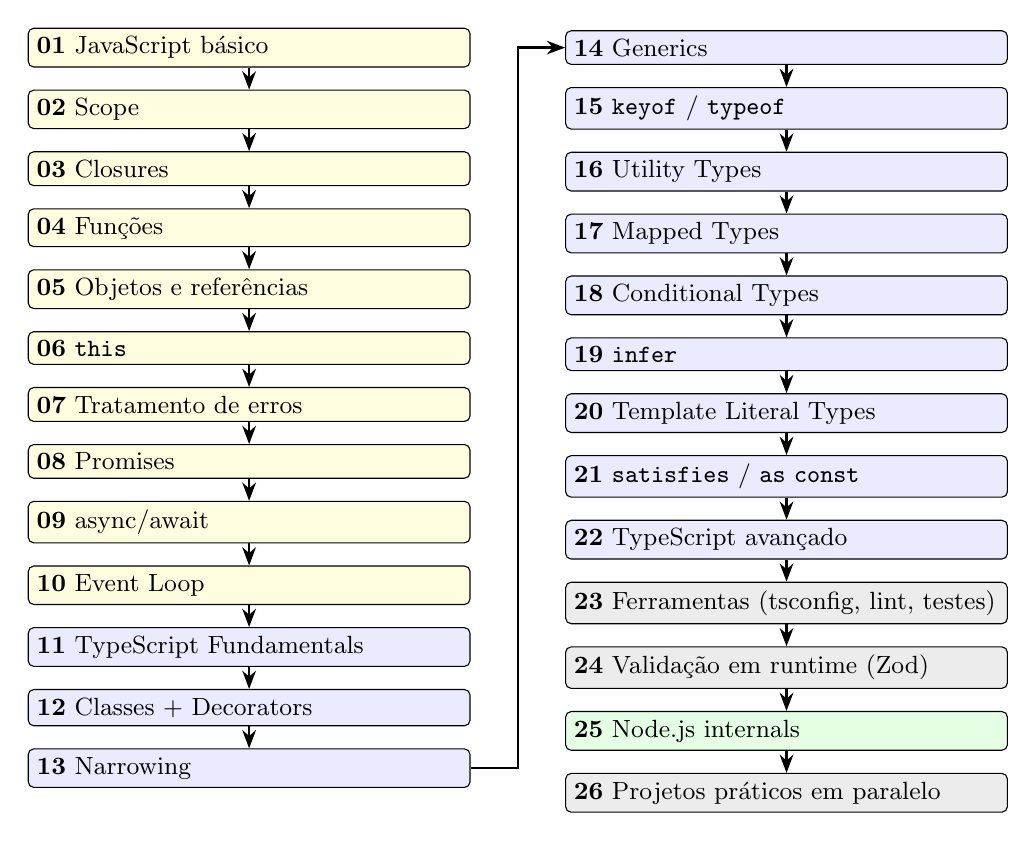
\begin{tikzpicture}[
  js/.style={draw, rounded corners=2pt, fill=yellow!12, text width=5.4cm, align=left, font=\small, inner sep=3pt},
  ts/.style={draw, rounded corners=2pt, fill=blue!8, text width=5.4cm, align=left, font=\small, inner sep=3pt},
  fe/.style={draw, rounded corners=2pt, fill=gray!15, text width=5.4cm, align=left, font=\small, inner sep=3pt},
  nd/.style={draw, rounded corners=2pt, fill=green!10, text width=5.4cm, align=left, font=\small, inner sep=3pt},
  node distance=0.28cm]
  \node[js] (s1) {\textbf{01} JavaScript básico};
  \node[js, below=of s1] (s2) {\textbf{02} Scope};
  \node[js, below=of s2] (s3) {\textbf{03} Closures};
  \node[js, below=of s3] (s4) {\textbf{04} Funções};
  \node[js, below=of s4] (s5) {\textbf{05} Objetos e referências};
  \node[js, below=of s5] (s6) {\textbf{06} \texttt{this}};
  \node[js, below=of s6] (s7) {\textbf{07} Tratamento de erros};
  \node[js, below=of s7] (s8) {\textbf{08} Promises};
  \node[js, below=of s8] (s9) {\textbf{09} async/await};
  \node[js, below=of s9] (s10) {\textbf{10} Event Loop};
  \node[ts, below=of s10] (s11) {\textbf{11} TypeScript Fundamentals};
  \node[ts, below=of s11] (s12) {\textbf{12} Classes + Decorators};
  \node[ts, below=of s12] (s13) {\textbf{13} Narrowing};
  \node[ts, right=1.2cm of s1] (s14) {\textbf{14} Generics};
  \node[ts, below=of s14] (s15) {\textbf{15} \texttt{keyof} / \texttt{typeof}};
  \node[ts, below=of s15] (s16) {\textbf{16} Utility Types};
  \node[ts, below=of s16] (s17) {\textbf{17} Mapped Types};
  \node[ts, below=of s17] (s18) {\textbf{18} Conditional Types};
  \node[ts, below=of s18] (s19) {\textbf{19} \texttt{infer}};
  \node[ts, below=of s19] (s20) {\textbf{20} Template Literal Types};
  \node[ts, below=of s20] (s21) {\textbf{21} \texttt{satisfies} / \texttt{as const}};
  \node[ts, below=of s21] (s22) {\textbf{22} TypeScript avançado};
  \node[fe, below=of s22] (s23) {\textbf{23} Ferramentas (tsconfig, lint, testes)};
  \node[fe, below=of s23] (s24) {\textbf{24} Validação em runtime (Zod)};
  \node[nd, below=of s24] (s25) {\textbf{25} Node.js internals};
  \node[fe, below=of s25] (s26) {\textbf{26} Projetos práticos em paralelo};
  \foreach \a/\b in {s1/s2,s2/s3,s3/s4,s4/s5,s5/s6,s6/s7,s7/s8,s8/s9,s9/s10,s10/s11,s11/s12,s12/s13,s14/s15,s15/s16,s16/s17,s17/s18,s18/s19,s19/s20,s20/s21,s21/s22,s22/s23,s23/s24,s24/s25,s25/s26}
    \draw[seta] (\a) -- (\b);
  \draw[seta] (s13.east) -- ++(0.6,0) |- (s14.west);
\end{tikzpicture}
\caption{Sequência de estudo. Amarelo: JavaScript. Azul: TypeScript. Cinza: ferramentas e prática. Verde: Node.js.}
\end{figure}

\begin{nota}[Em paralelo, não em série]
Os passos 01--10 não precisam terminar antes do 11. Uma cadência que funciona: em cada sessão de estudo, um tópico TS novo mais a revisão do tópico JS que ele usa (tabela do Capítulo~2). Faça rápido o que já sabe e gaste tempo real em closures, \code{this} e Event Loop. O passo 26 começa no primeiro dia.
\end{nota}

% =====================================================================
\chapter{Checklist de domínio}
\label{cap:checklist}

Critérios observáveis: não ``estudei'', mas ``consigo fazer sem consultar''. Imprima este capítulo e revise mensalmente.

\section{JavaScript}

{\small
\begin{tabularx}{\textwidth}{@{}clXr@{}}
\toprule
 & \textbf{Tópico} & \textbf{Você domina quando consegue\ldots} & \textbf{Seção} \\
\midrule
\cb & Scope & explicar TDZ e a diferença entre \code{let}, \code{const} e \code{var} & \ref{sec:scope} \\
\cb & Closures & explicar o \code{3 3 3} do loop com \code{var} e desenhar o ambiente capturado & \ref{sec:closures} \\
\cb & Factory Functions & implementar uma factory com estado privado sem hesitar & \ref{sec:closures} \\
\cb & \code{this} & prever o valor de \code{this} em qualquer call site & \ref{sec:this} \\
\cb & Arrow Functions & dizer quando \emph{não} usar arrow & \ref{sec:this} \\
\cb & Objects / References & encontrar uma mutação acidental por referência compartilhada & \ref{sec:objetos} \\
\cb & Destructuring & desestruturar aninhado com renomeação, default e rest & \ref{sec:objetos} \\
\cb & Spread / Rest & distinguir cópia rasa de profunda e usar rest em parâmetros & \ref{sec:funcoes} \\
\cb & Array methods & usar \code{reduce} sem consultar e saber quais métodos mutam & \ref{sec:arrays} \\
\cb & Tratamento de erros & criar erros customizados corretamente, com \code{cause} & \ref{sec:erros} \\
\cb & \code{?.} e \code{??} & escolher entre \code{??} e \code{||} pelo significado de \code{0} e \code{''} & \ref{sec:nullish} \\
\cb & Promises & usar \code{allSettled} quando apropriado & \ref{sec:promises} \\
\cb & Async/Await & paralelizar awaits independentes e tratar erros corretamente & \ref{sec:async} \\
\cb & Event Loop & explicar a ordem de micro e macrotasks & \ref{sec:eventloop} \\
\cb & Prototype & desenhar a prototype chain de uma hierarquia de classes & \ref{sec:prototype} \\
\cb & Map / Set / WeakMap / WeakSet & justificar cada um no lugar de objetos e arrays & \ref{sec:jsmedia} \\
\cb & ESM / CommonJS & configurar ESM do zero e explicar um ciclo de dependência & \ref{sec:jsmedia} \\
\bottomrule
\end{tabularx}
}

\section{TypeScript}

{\small
\begin{tabularx}{\textwidth}{@{}clXr@{}}
\toprule
 & \textbf{Tópico} & \textbf{Você domina quando consegue\ldots} & \textbf{Seção} \\
\midrule
\cb & Unions / Intersections & modelar estados como union de literais e compor com \code{\&} & \ref{sec:tsfund} \\
\cb & Classes + Decorators & escrever hierarquias com \code{abstract}/\code{override} e um decorator simples & \ref{sec:classes} \\
\cb & Narrowing & usar \code{typeof}, \code{in}, \code{instanceof} e igualdade sem assertions & \ref{sec:narrowing} \\
\cb & Type Guards & escrever predicates corretos e discriminated unions & \ref{sec:narrowing} \\
\cb & Assertion Functions & escrever \code{asserts x is T} para validar pré-condições & \ref{sec:narrowing} \\
\cb & Generics & escrever constraints sem consultar & \ref{sec:generics} \\
\cb & \code{keyof}, \code{typeof}, indexed access & derivar tipos de valores e diferenciar do \code{typeof} de runtime & \ref{sec:keyof} \\
\cb & Utility Types & derivar DTOs de criação, atualização e resposta de um único tipo & \ref{sec:utility} \\
\cb & Mapped Types & reescrever \code{Partial} e usar key remapping & \ref{sec:mapped} \\
\cb & Conditional Types & explicar distributividade e reimplementar \code{Exclude} & \ref{sec:conditional} \\
\cb & \code{infer} & reimplementar \code{ReturnType} e \code{Awaited} & \ref{sec:infer} \\
\cb & Template Literal Types & tipar parâmetros de rota ou \code{Path<T>} & \ref{sec:template} \\
\cb & \code{satisfies} & saber quando preferir \code{satisfies}, \code{as const} ou anotação & \ref{sec:satisfies} \\
\cb & \code{unknown} / \code{never} & validar entradas externas e usar exhaustive checks & \ref{sec:unknown} \\
\cb & Function Overloads & decidir entre overload, union e generic & \ref{sec:overloads} \\
\cb & Structural Typing & explicar excess property checks e usar branded types & \ref{sec:structural} \\
\cb & Variance & explicar por que parâmetros são contravariantes & \ref{cap:tsavancado} \\
\cb & \code{.d.ts} & escrever declarações próprias para uma lib sem tipos & \ref{cap:tsavancado} \\
\cb & Module Augmentation & adicionar campos ao request do seu framework & \ref{cap:tsavancado} \\
\cb & Advanced \code{tsconfig} & configurar um projeto strict do zero & \ref{sec:tsconfig} \\
\cb & Type tests & escrever testes de tipos com \code{expect-type} ou Vitest & \ref{cap:ferramentas} \\
\bottomrule
\end{tabularx}
}

\section{Ferramentas e ecossistema}

{\small
\begin{tabularx}{\textwidth}{@{}cX@{}}
\toprule
\cb & Configuro ESLint (\code{typescript-eslint} type-aware) + Prettier + TS em um projeto novo \\
\cb & Escrevo testes com Vitest ou Jest, com mocks tipados \\
\cb & Valido input HTTP e variáveis de ambiente com Zod \\
\cb & Configuro um ORM tipado (Prisma ou Drizzle) com migrations \\
\cb & Faço build com \code{tsup} ou \code{esbuild} e checo tipos com \code{tsc --noEmit} no CI \\
\bottomrule
\end{tabularx}
}

\section{Node.js}

{\small
\begin{tabularx}{\textwidth}{@{}cX@{}}
\toprule
\cb & Diagnostico bloqueio do Event Loop em um serviço real \\
\cb & Processo arquivos grandes com Streams e \code{pipeline()}, respeitando backpressure \\
\cb & Movo trabalho CPU-bound para Worker Threads \\
\cb & Implemento graceful shutdown com \code{SIGTERM} \\
\cb & Propago contexto de requisição com \code{AsyncLocalStorage} \\
\cb & Tenho logs estruturados, métricas e traces básicos (observabilidade) \\
\bottomrule
\end{tabularx}
}

\begin{nota}[Teste final de domínio]
Pegue um módulo real do seu backend (controller + service + repositório) e: (1) remova todo \code{any}; (2) derive os DTOs com utility types; (3) valide o input com um schema; (4) modele estados com discriminated union e exhaustive check; (5) explique, em voz alta e linha a linha, o que acontece em runtime quando uma requisição chega.
\end{nota}

% =====================================================================
\chapter{Regras do roadmap}

\begin{enumerate}
  \item \textbf{Não tente terminar JavaScript antes de começar TypeScript.}\\
  JavaScript não tem fim. Se esperar dominá-lo por completo, você nunca começa o que realmente queria aprender.

  \item \textbf{Aprenda TypeScript e aprofunde JavaScript conforme os conceitos aparecerem.}\\
  Cada dúvida de runtime que surge no TS indica qual tópico de JS estudar agora.

  \item \textbf{O objetivo não é decorar APIs, mas entender por que o código funciona.}\\
  A documentação resolve a assinatura de \code{reduce}. Ela não resolve a dúvida sobre por que o \code{this} sumiu.

  \item \textbf{TypeScript ajuda em compile time; JavaScript determina o comportamento em runtime.}\\
  Tipos descrevem expectativas. Validação, closures, Promises e o Event Loop decidem o que acontece de fato.

  \item \textbf{Se você não sabe explicar em voz alta, você não domina.}\\
  Explicar para outra pessoa (ou para o pato de borracha) expõe as lacunas que a leitura esconde.

  \item \textbf{Um projeto real vale mais que dez tutoriais concluídos.}\\
  Tutoriais mostram o caminho feliz; projetos mostram os erros, as integrações e as decisões.
\end{enumerate}

% =====================================================================
\appendix
\chapter{Referências e Leitura Adicional}

\section*{Documentação oficial}
\begin{itemize}
  \item \textbf{TypeScript Handbook} --- \url{https://www.typescriptlang.org/docs/handbook/}
  \item \textbf{TSConfig Reference} --- \url{https://www.typescriptlang.org/tsconfig/}
  \item \textbf{TypeScript Release Notes} --- \url{https://www.typescriptlang.org/docs/handbook/release-notes/overview.html}
  \item \textbf{TypeScript Playground} (veja o JS emitido ao lado do TS) --- \url{https://www.typescriptlang.org/play}
  \item \textbf{MDN Web Docs --- JavaScript} --- \url{https://developer.mozilla.org/en-US/docs/Web/JavaScript}
  \item \textbf{Node.js --- The Node.js Event Loop} --- \url{https://nodejs.org/en/learn/asynchronous-work/event-loop-timers-and-nexttick}
  \item \textbf{Node.js API Documentation} --- \url{https://nodejs.org/api/}
\end{itemize}

\section*{Livros}
\begin{itemize}
  \item Boris Cherny, \emph{Programming TypeScript}, O'Reilly.
  \item Dan Vanderkam, \emph{Effective TypeScript}, O'Reilly.
  \item Kyle Simpson, \emph{You Don't Know JS Yet} (leia seletivamente: scope, closures, \code{this}, prototypes) --- \url{https://github.com/getify/You-Dont-Know-JS}
\end{itemize}

\section*{Prática e comunidade}
\begin{itemize}
  \item \textbf{type-challenges} --- \url{https://github.com/type-challenges/type-challenges}
  \item \textbf{tsconfig/bases} (configurações de referência) --- \url{https://github.com/tsconfig/bases}
  \item \textbf{Total TypeScript} (Matt Pocock) --- \url{https://www.totaltypescript.com}
  \item Newsletter \textbf{TypeScript Weekly}.
  \item Canais: Matt Pocock, Theo, Web Dev Simplified.
\end{itemize}

\chapter{Glossário}

\begin{description}
  \item[Type erasure\index{type erasure}] remoção das anotações de tipo na compilação; o JS gerado não contém tipos.
  \item[Lexical environment\index{lexical environment}] estrutura que mapeia nomes a valores em um escopo, com referência para o escopo externo.
  \item[Closure\index{closure}] função que retém acesso ao escopo léxico onde foi criada.
  \item[Hoisting\index{hoisting}] elevação de declarações ao topo do escopo antes da execução.
  \item[TDZ\index{TDZ}] Temporal Dead Zone: período entre o início do bloco e a inicialização de \code{let}/\code{const}.
  \item[Factory function\index{factory function}] função que cria e retorna objetos, geralmente com estado privado via closure.
  \item[Call site] o ponto onde uma função é chamada; determina o valor de \code{this}\index{this}.
  \item[Shallow copy\index{shallow copy}] cópia que duplica apenas o primeiro nível de um objeto.
  \item[Prototype chain\index{prototype chain}] cadeia de objetos usada na resolução de propriedades.
  \item[Microtask / Macrotask] filas distintas do Event Loop\index{Event Loop}, com prioridades diferentes.
  \item[libuv\index{libuv}] biblioteca em C que implementa o Event Loop e o thread pool do Node.js.
  \item[Narrowing\index{narrowing}] redução do tipo de um valor a partir de uma checagem em runtime.
  \item[Type guard] função cujo retorno é \code{x is Y}.
  \item[Assertion function] função com retorno \code{asserts x is Y}; lança erro se a condição falhar.
  \item[Discriminated union\index{discriminated union}] union de objetos com um campo literal comum que identifica cada variante.
  \item[Generics\index{generics}] parâmetros de tipo que relacionam entradas e saídas.
  \item[Generic constraint] restrição aplicada a um parâmetro de tipo via \code{extends}.
  \item[Utility types\index{utility types}] tipos da biblioteca padrão que transformam outros tipos.
  \item[Mapped type\index{mapped types}] tipo derivado iterando sobre as chaves de outro tipo.
  \item[Conditional type\index{conditional types}] tipo que resolve com base em \code{T extends U ? X : Y}.
  \item[Distributividade\index{distributividade}] aplicação automática de um conditional type a cada membro de uma union.
  \item[infer\index{infer}] extrai um tipo dentro de um conditional type.
  \item[Template literal type\index{template literal types}] tipo de string construído com a sintaxe de template.
  \item[satisfies\index{satisfies}] operador que valida a forma preservando o tipo inferido.
  \item[unknown\index{unknown}] tipo seguro para valores desconhecidos; exige narrowing antes do uso.
  \item[never\index{never}] tipo sem valores; usado em exhaustive checks.
  \item[Decorator\index{decorators}] função que modifica ou anota classes, métodos e propriedades.
  \item[Structural typing\index{structural typing}] tipagem por forma, não por nome.
  \item[Variance\index{variance}] como subtipos se relacionam em posições covariantes e contravariantes.
  \item[Branded type\index{branded types}] tipo nominal simulado por uma marca única.
  \item[Declaration merging\index{declaration merging}] fusão de declarações com o mesmo nome.
  \item[Module augmentation\index{module augmentation}] extensão de um módulo existente a partir de outro arquivo.
  \item[ESM / CommonJS\index{ESM}\index{CommonJS}] os dois sistemas de módulos do Node.js.
  \item[tsconfig\index{tsconfig}] arquivo de configuração do compilador TypeScript.
  \item[Validação em runtime\index{validação em runtime}] verificação de dados externos durante a execução, por exemplo com Zod.
  \item[Tratamento de erros\index{tratamento de erros}] estratégia para lançar, capturar, relançar e reportar falhas.
\end{description}

\chapter{FAQ e erros comuns}

\section*{Por que \texttt{any} é ruim se funciona?}
Porque desliga o sistema de tipos para aquele valor --- e para tudo o que deriva dele. O código compila, mas você perde as garantias que o TypeScript existe para dar. Use \code{unknown} quando não souber o tipo.

\section*{Quando usar \texttt{interface} e quando usar \texttt{type}?}
\code{interface} para contratos de objeto que podem ser estendidos ou mesclados. \code{type} para unions, interseções, aliases de primitivos e tipos compostos.

\section*{Por que meu \texttt{this} está \texttt{undefined}?}
Porque a função foi chamada isoladamente (não como método) e você está em strict mode --- o caso típico é passar um método como callback. Use \code{bind} ou uma arrow function para preservar o \code{this} (Seção~\ref{sec:this}).

\section*{Por que o Zod não substitui o TypeScript?}
Zod valida em \textbf{runtime}; TypeScript checa em \textbf{compile time}. São complementares: o Zod verifica dados externos (HTTP, env, banco) e infere os tipos que o TS usa no resto do código.

\section*{Por que a Promise não é cancelável?}
Porque uma Promise representa um resultado que já está sendo produzido. Para cancelar o trabalho, use \code{AbortController} e APIs que aceitam \code{signal} (\code{fetch}, \code{setTimeout} de \code{node:timers/promises}, streams).

\section*{Por que \texttt{Promise.all} rejeita tudo se uma falhar?}
Porque ele é ``tudo ou nada''. Para coletar sucessos e falhas individualmente, use \code{Promise.allSettled}.

\section*{Por que \texttt{Object.keys} retorna \texttt{string[]} e não \texttt{(keyof T)[]}?}
Por causa da tipagem estrutural: um objeto do tipo \code{T} pode ter propriedades extras em runtime, então o TypeScript não pode garantir que todas as chaves sejam \code{keyof T} (Seção~\ref{sec:keyof}).

\section*{Por que o \texttt{tsc} passa, mas o import com alias quebra em runtime?}
Porque \code{paths} só existe em compile time; o \code{tsc} não reescreve os imports no JS emitido (Seção~\ref{sec:tsconfig}).

\section*{Meu \texttt{tsx} roda o código, então os tipos estão certos?}
Não. \code{tsx}, \code{esbuild}, \code{swc} e o type stripping do Node apenas apagam os tipos. Só o \code{tsc} checa (Capítulo~\ref{cap:ferramentas}).

\printindex

\end{document}
